\section{Результаты вычислений}

Вычислительные эксперименты проведены для трех тестовых функций:

\[
\begin{alignedat}{2}
    f_1(x) &= (x-2)^2+1, 
        &\quad x &\in [0,5];\\
    f_2(x) &= x^2+2\sin(3x), 
        &\quad x &\in [0.8,3];\\
    f_3(x) &= x^2+5\sin(2x)+2\cos(3x), 
        &\quad x &\in [-3,3].
\end{alignedat}
\]

Унимодальные функции $f_1$ и $f_2$ использовались для проверки локальных методов,
а многоэкстремальная $f_3$ --- для сравнения глобальных методов. В качестве критериев
оценки рассматривались найденная координата минимума, длина итогового
отрезка локализации, число вычислений функции и динамика сходимости.


\subsection{Работа локальных методов}

Для каждой локальной процедуры на рисунке показаны график функции на всем
интервале, точки вычислений, найденный минимум и увеличенная окрестность
итогового отрезка локализации.

\begin{figure}[H]
	\centering
	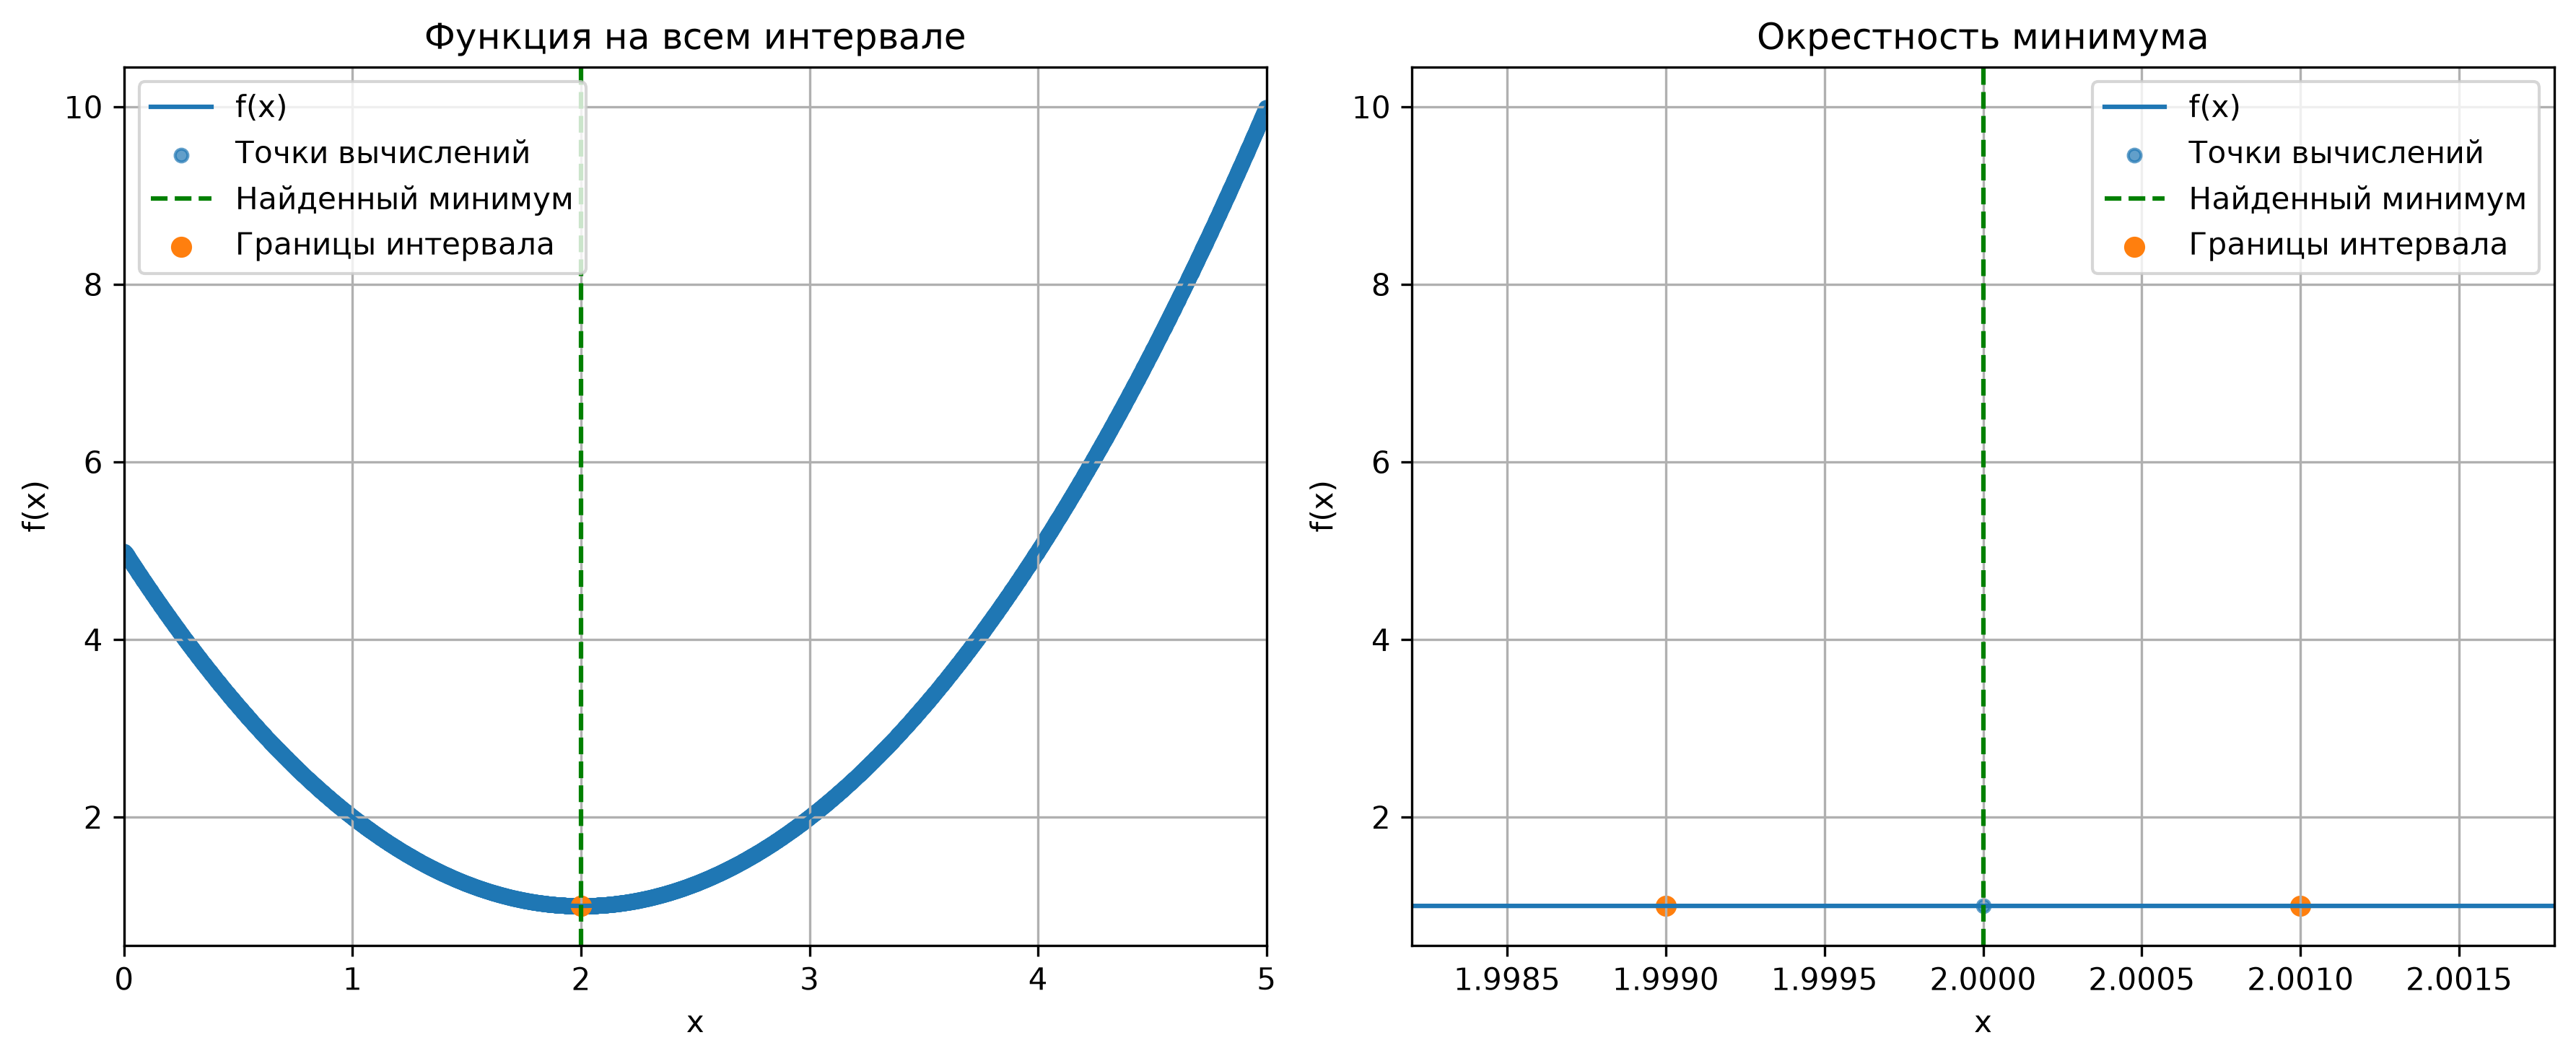
\includegraphics[width=0.95\textwidth]{results/passive/f1.png}
	\caption{Пассивный поиск на функции $f_1$.}
	\label{fig:passive-f1}
\end{figure}

\begin{figure}[H]
	\centering
	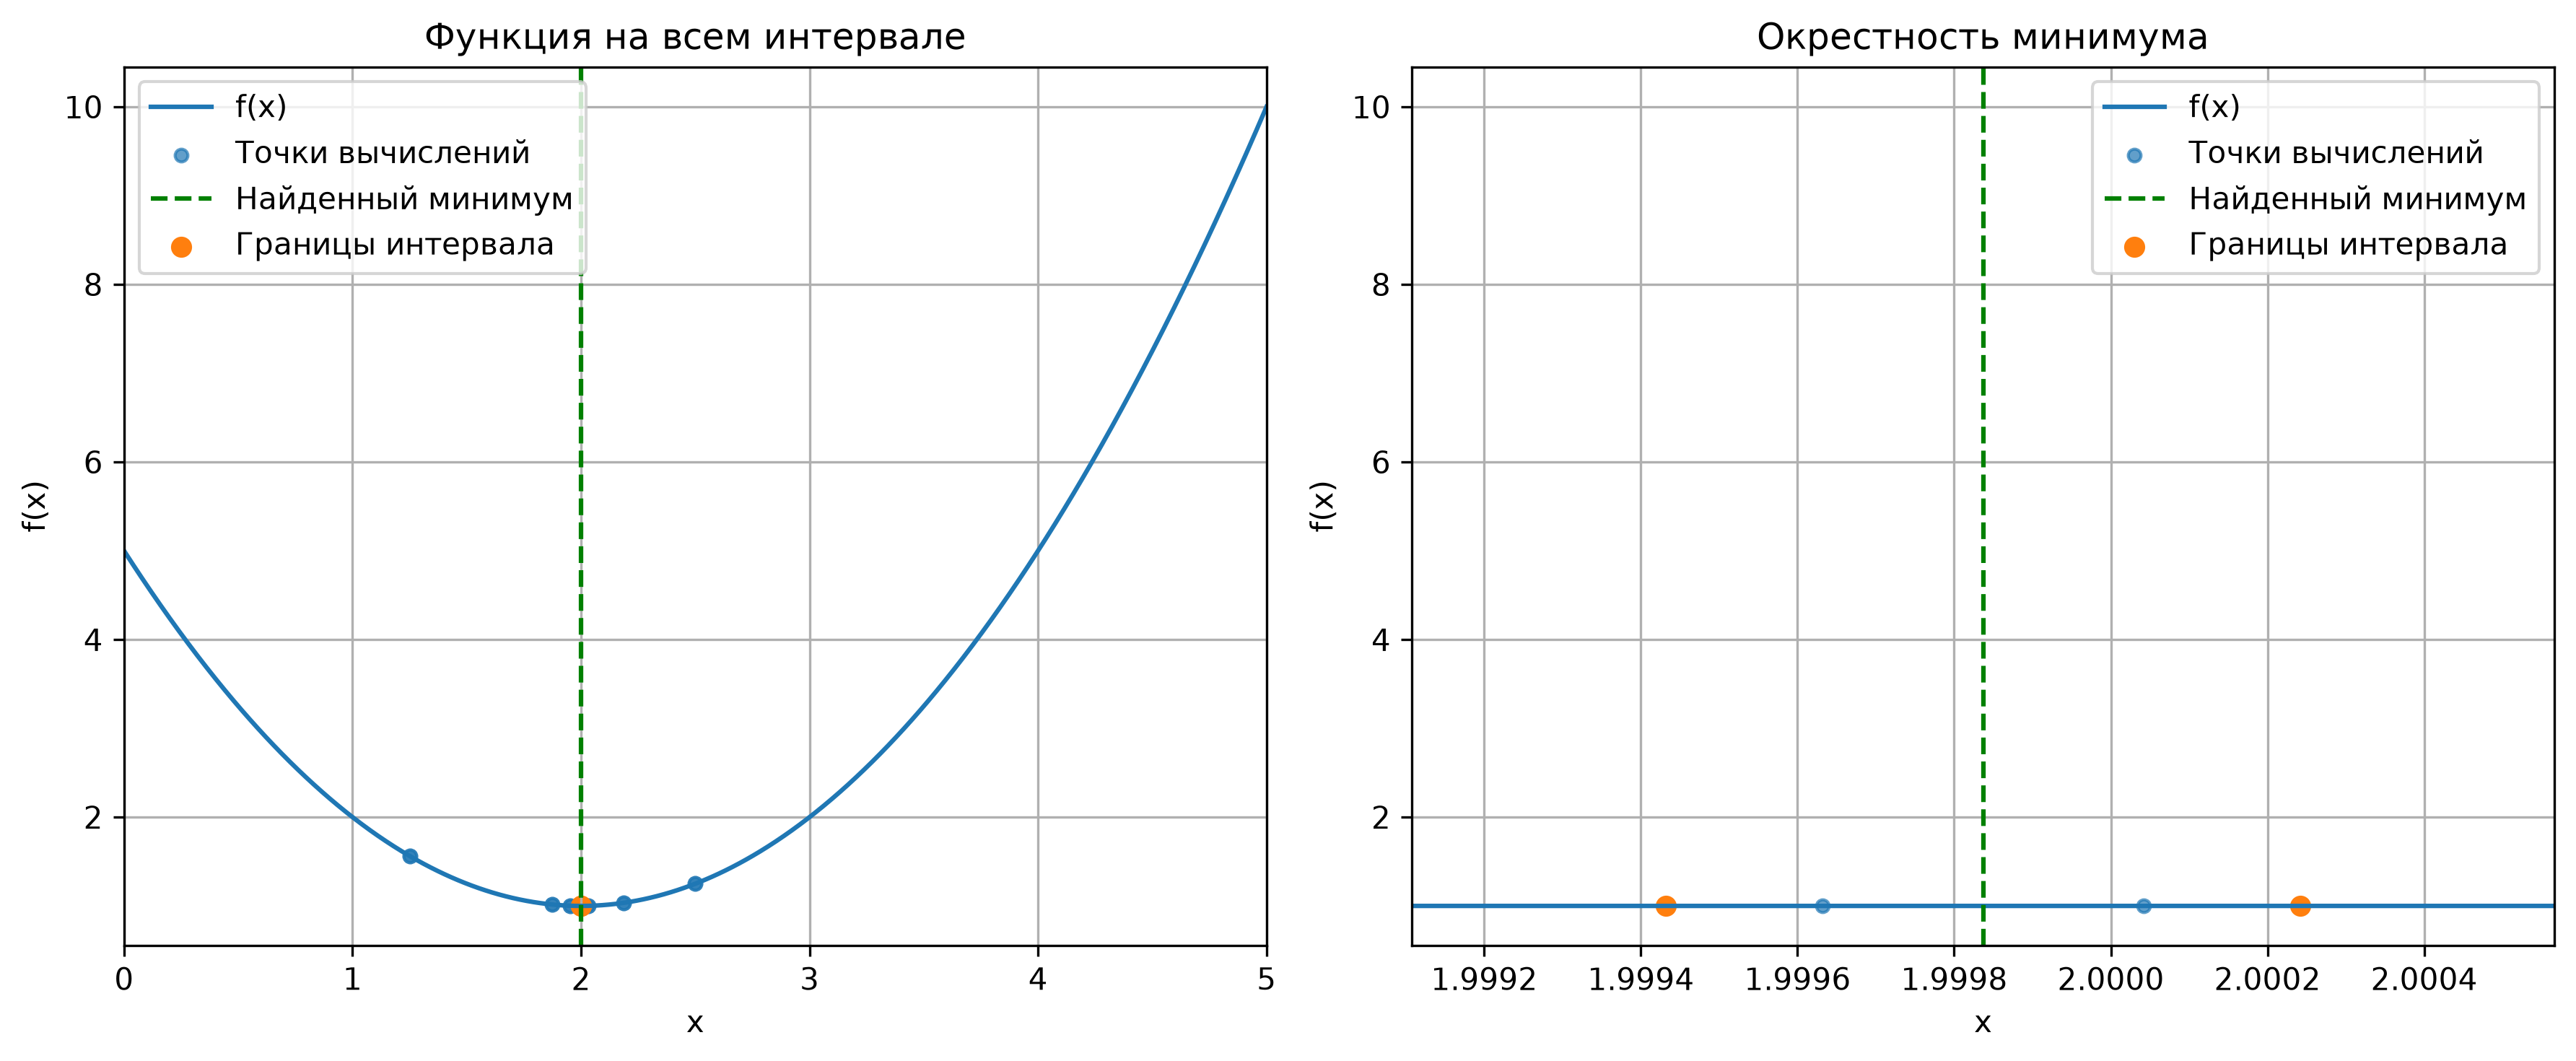
\includegraphics[width=0.95\textwidth]{results/dichotomy/f1.png}
	\caption{Метод дихотомии на функции $f_1$.}
	\label{fig:dichotomy-f1}
\end{figure}

\begin{figure}[H]
	\centering
	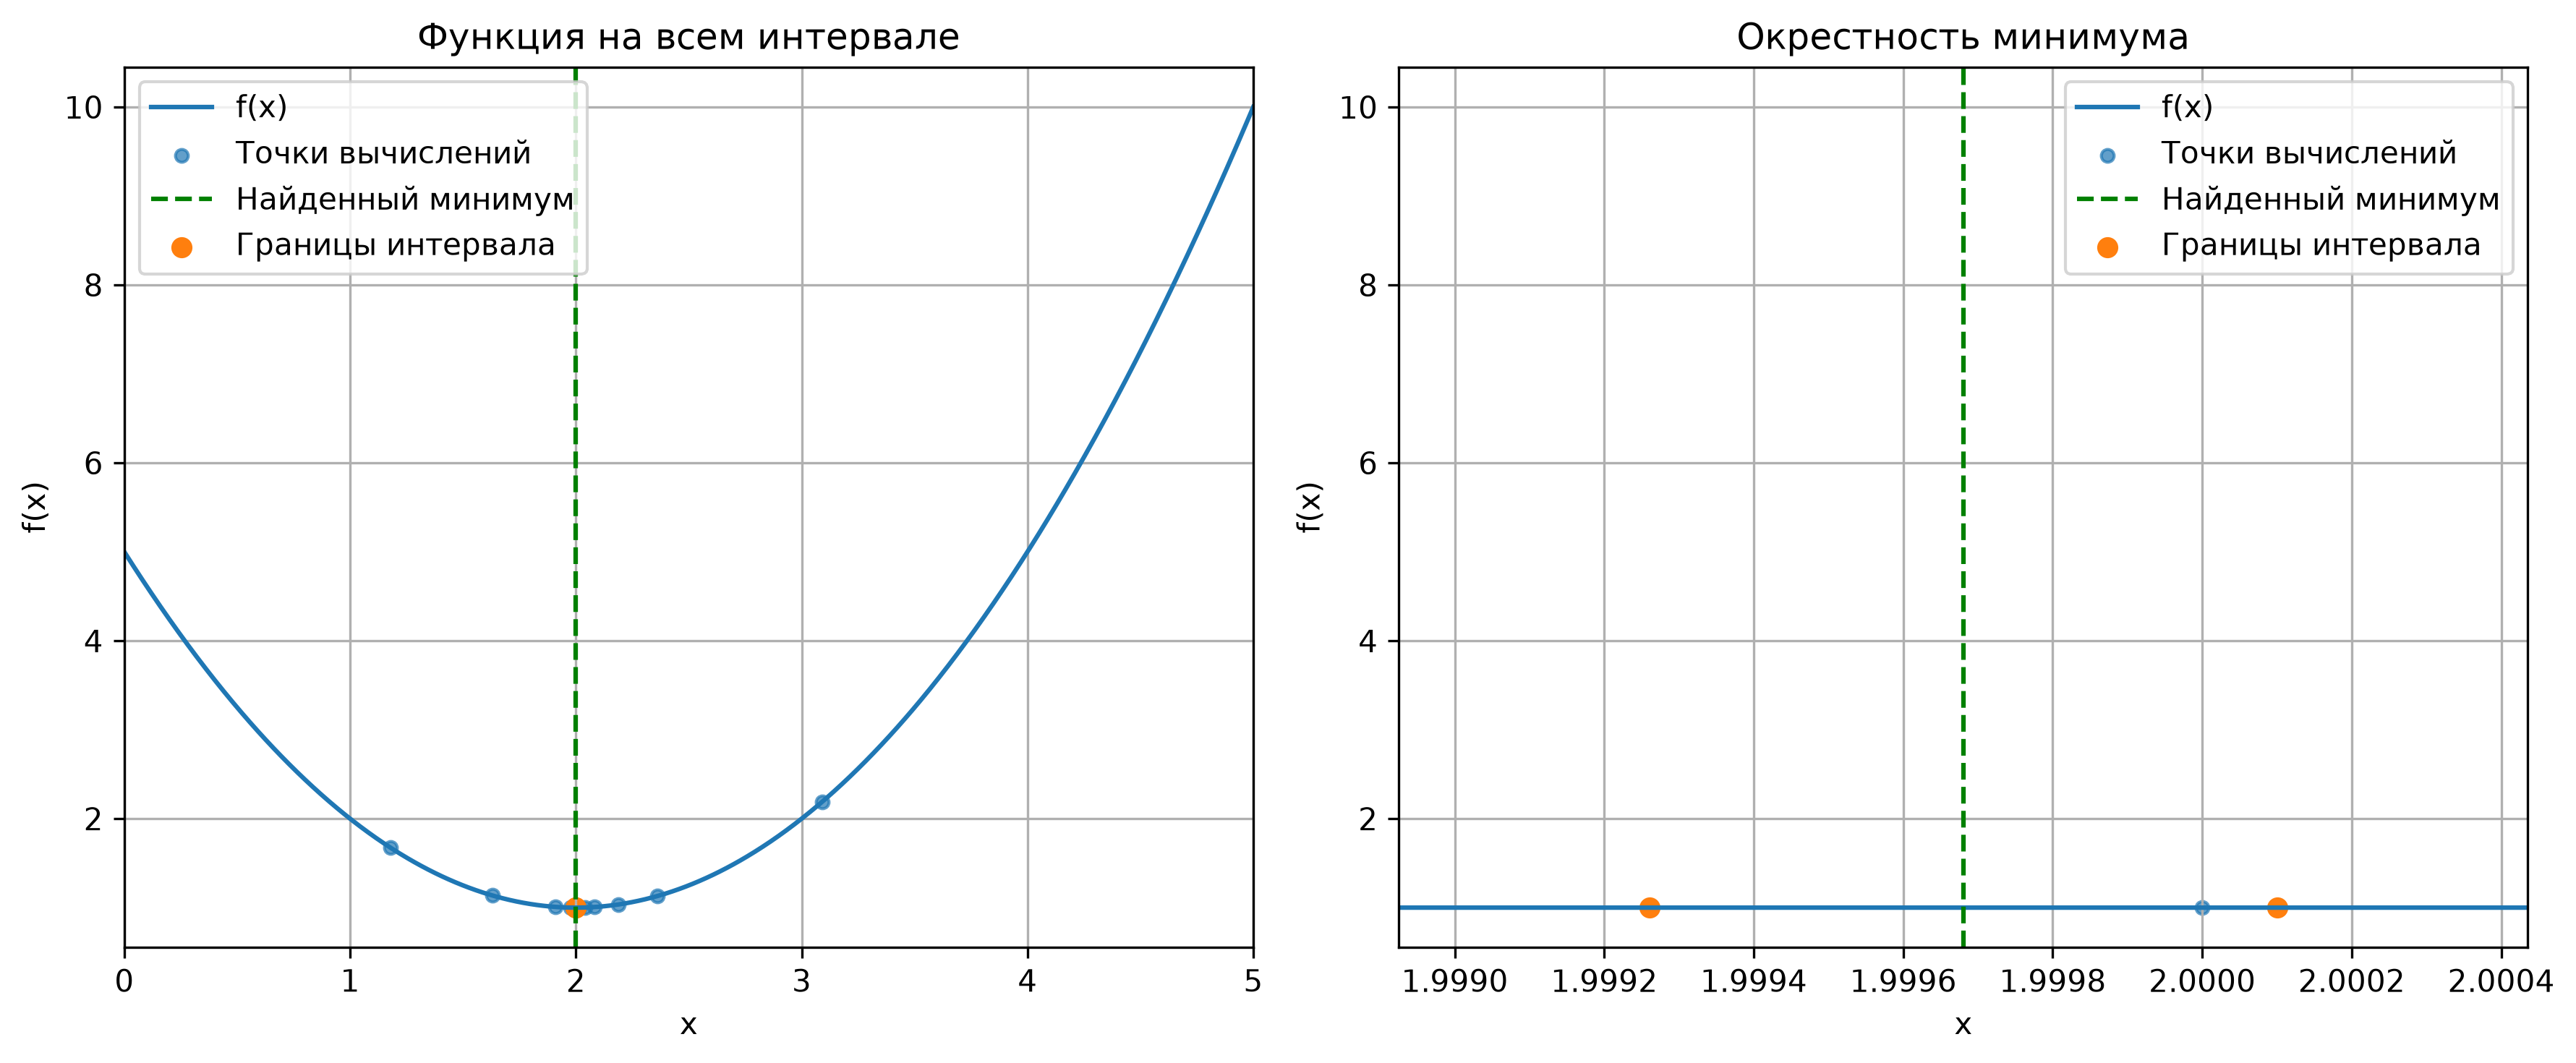
\includegraphics[width=0.95\textwidth]{results/fibonacci/f1.png}
	\caption{Метод Фибоначчи на функции $f_1$.}
	\label{fig:fibonacci-f1}
\end{figure}

\begin{figure}[H]
	\centering
	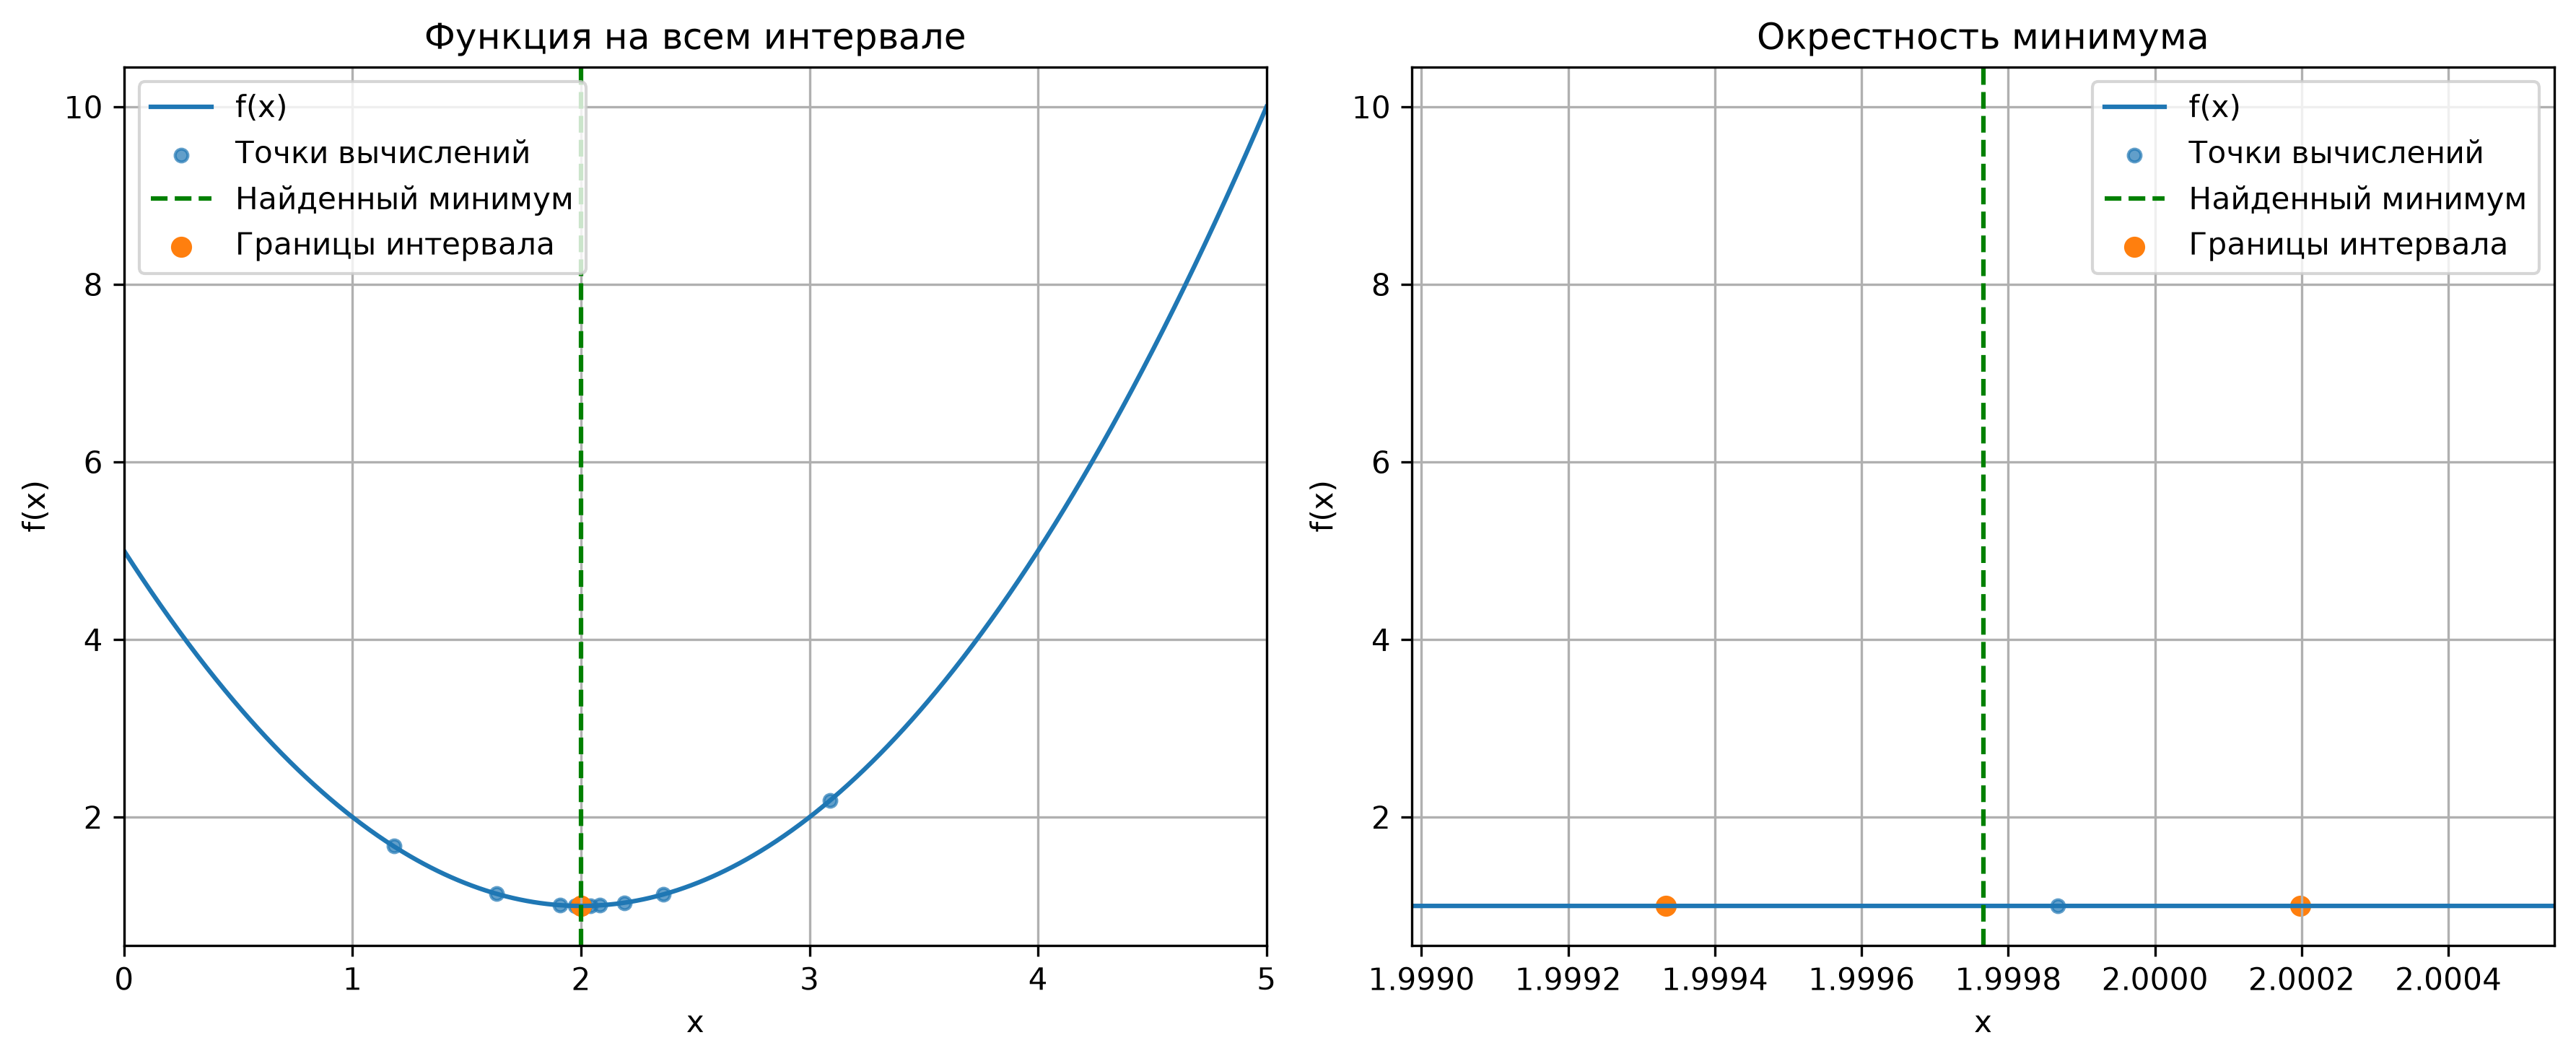
\includegraphics[width=0.95\textwidth]{results/golden_ratio/f1.png}
	\caption{Метод золотого сечения на функции $f_1$.}
	\label{fig:golden-f1}
\end{figure}

\begin{figure}[H]
	\centering
	
\includegraphics[width=0.95\textwidth]{results/parabola/f1.png}
	\caption{Метод парабол на функции $f_1$.}
	\label{fig:parabola-f1}
\end{figure}

На квадратичной функции $f_1$ все методы локализации демонстрируют ожидаемое
поведение: вычисления концентрируются около единственного минимума $x=2$.
Методы дихотомии, Фибоначчи и золотого сечения последовательно сужают интервал,
тогда как пассивный поиск равномерно исследует весь отрезок.

\begin{figure}[H]
	\centering
	
\includegraphics[width=0.95\textwidth]{results/passive/f2.png}
	\caption{Пассивный поиск на функции $f_2$.}
	\label{fig:passive-f2}
\end{figure}

\begin{figure}[H]
	\centering
	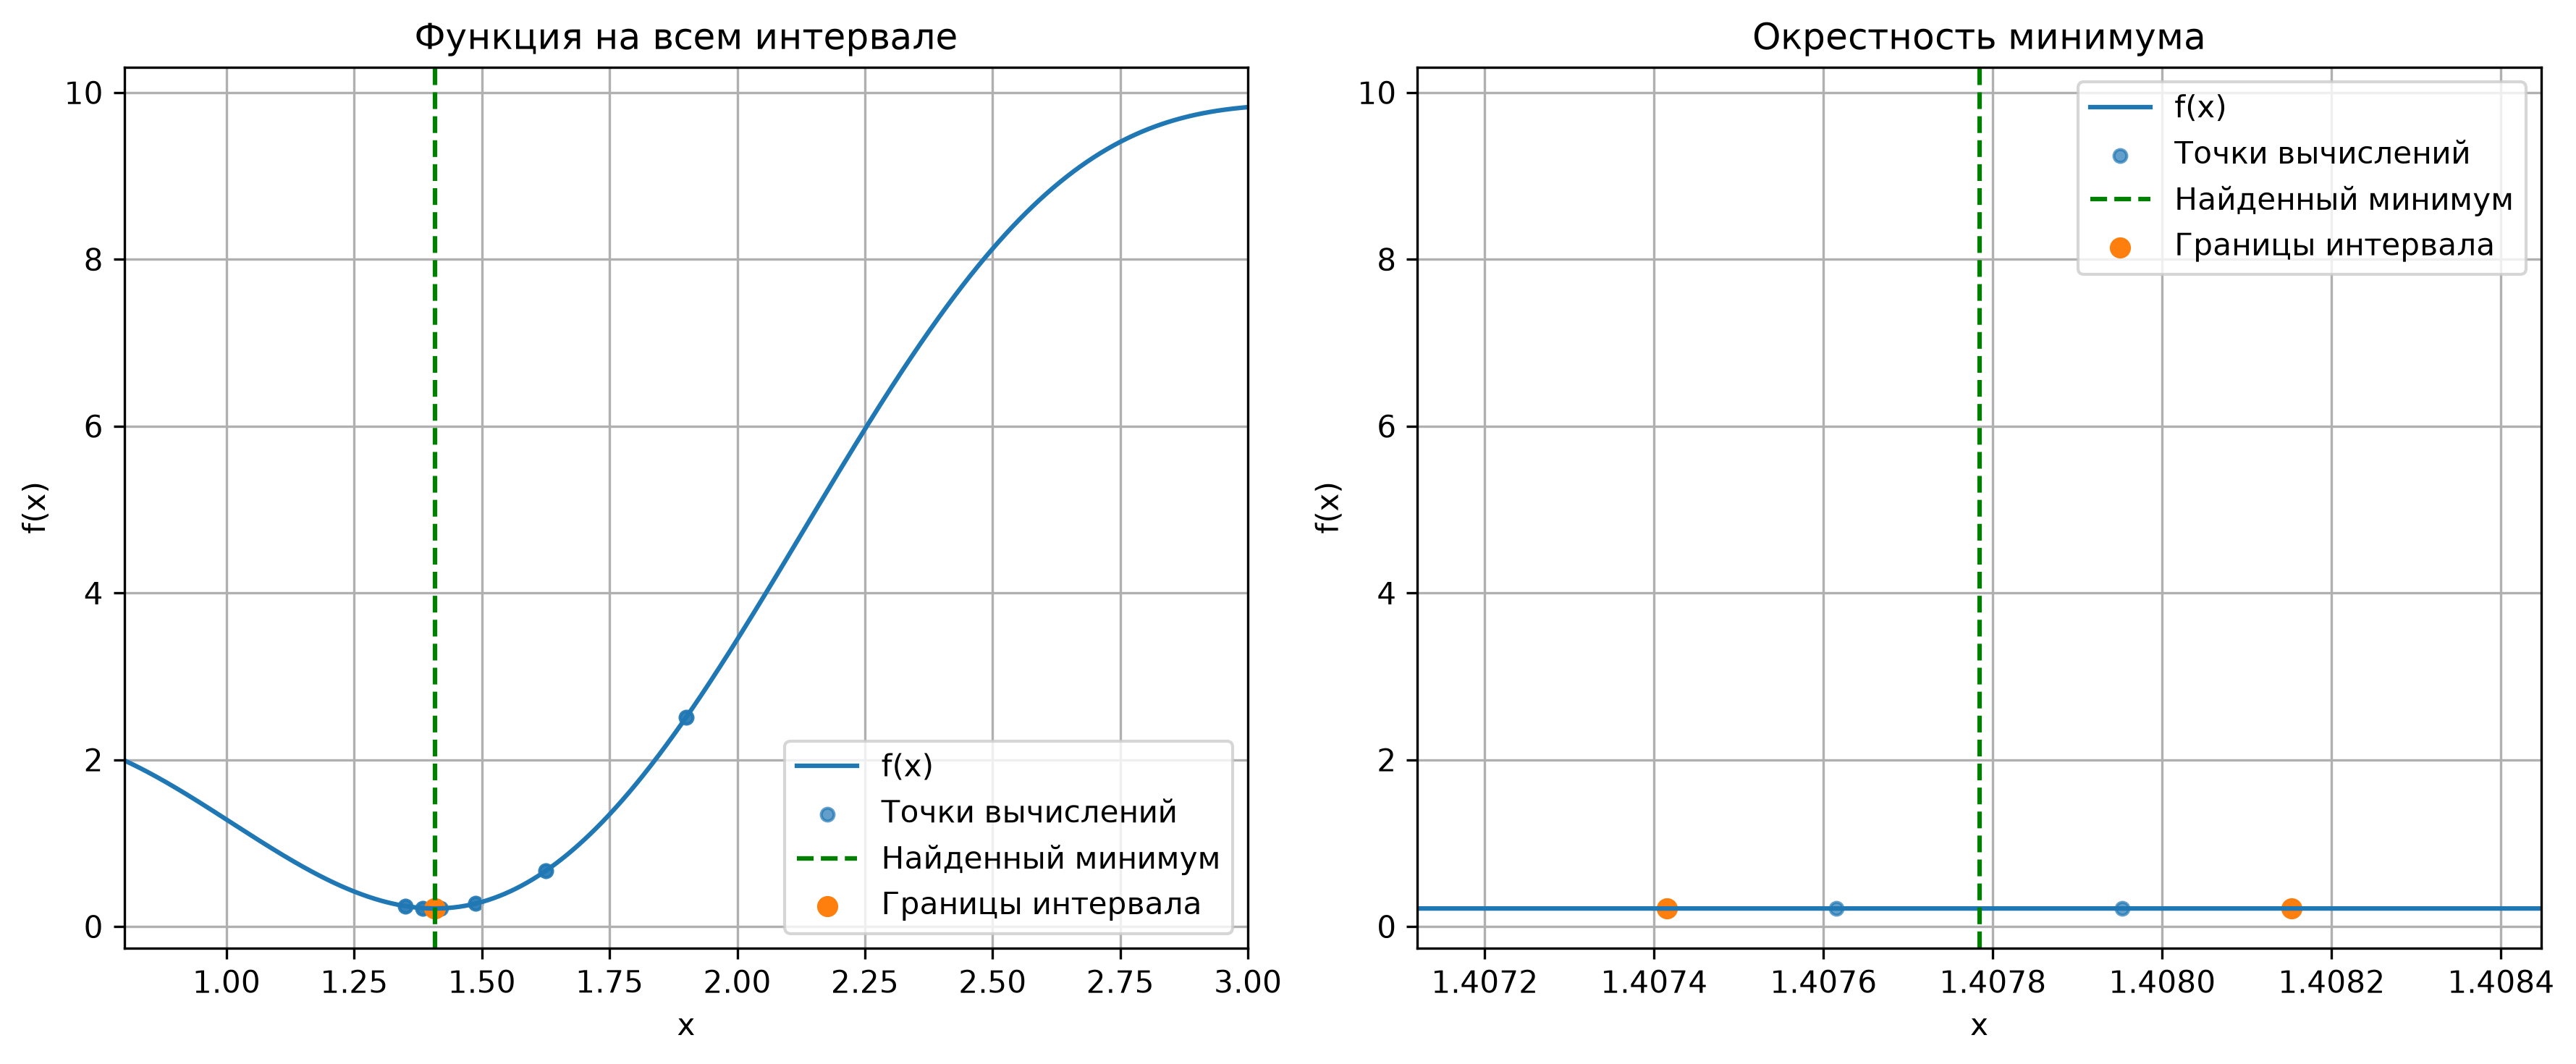
\includegraphics[width=0.95\textwidth]{results/dichotomy/f2.png}
	\caption{Метод дихотомии на функции $f_2$.}
	\label{fig:dichotomy-f2}
\end{figure}

\begin{figure}[H]
	\centering
	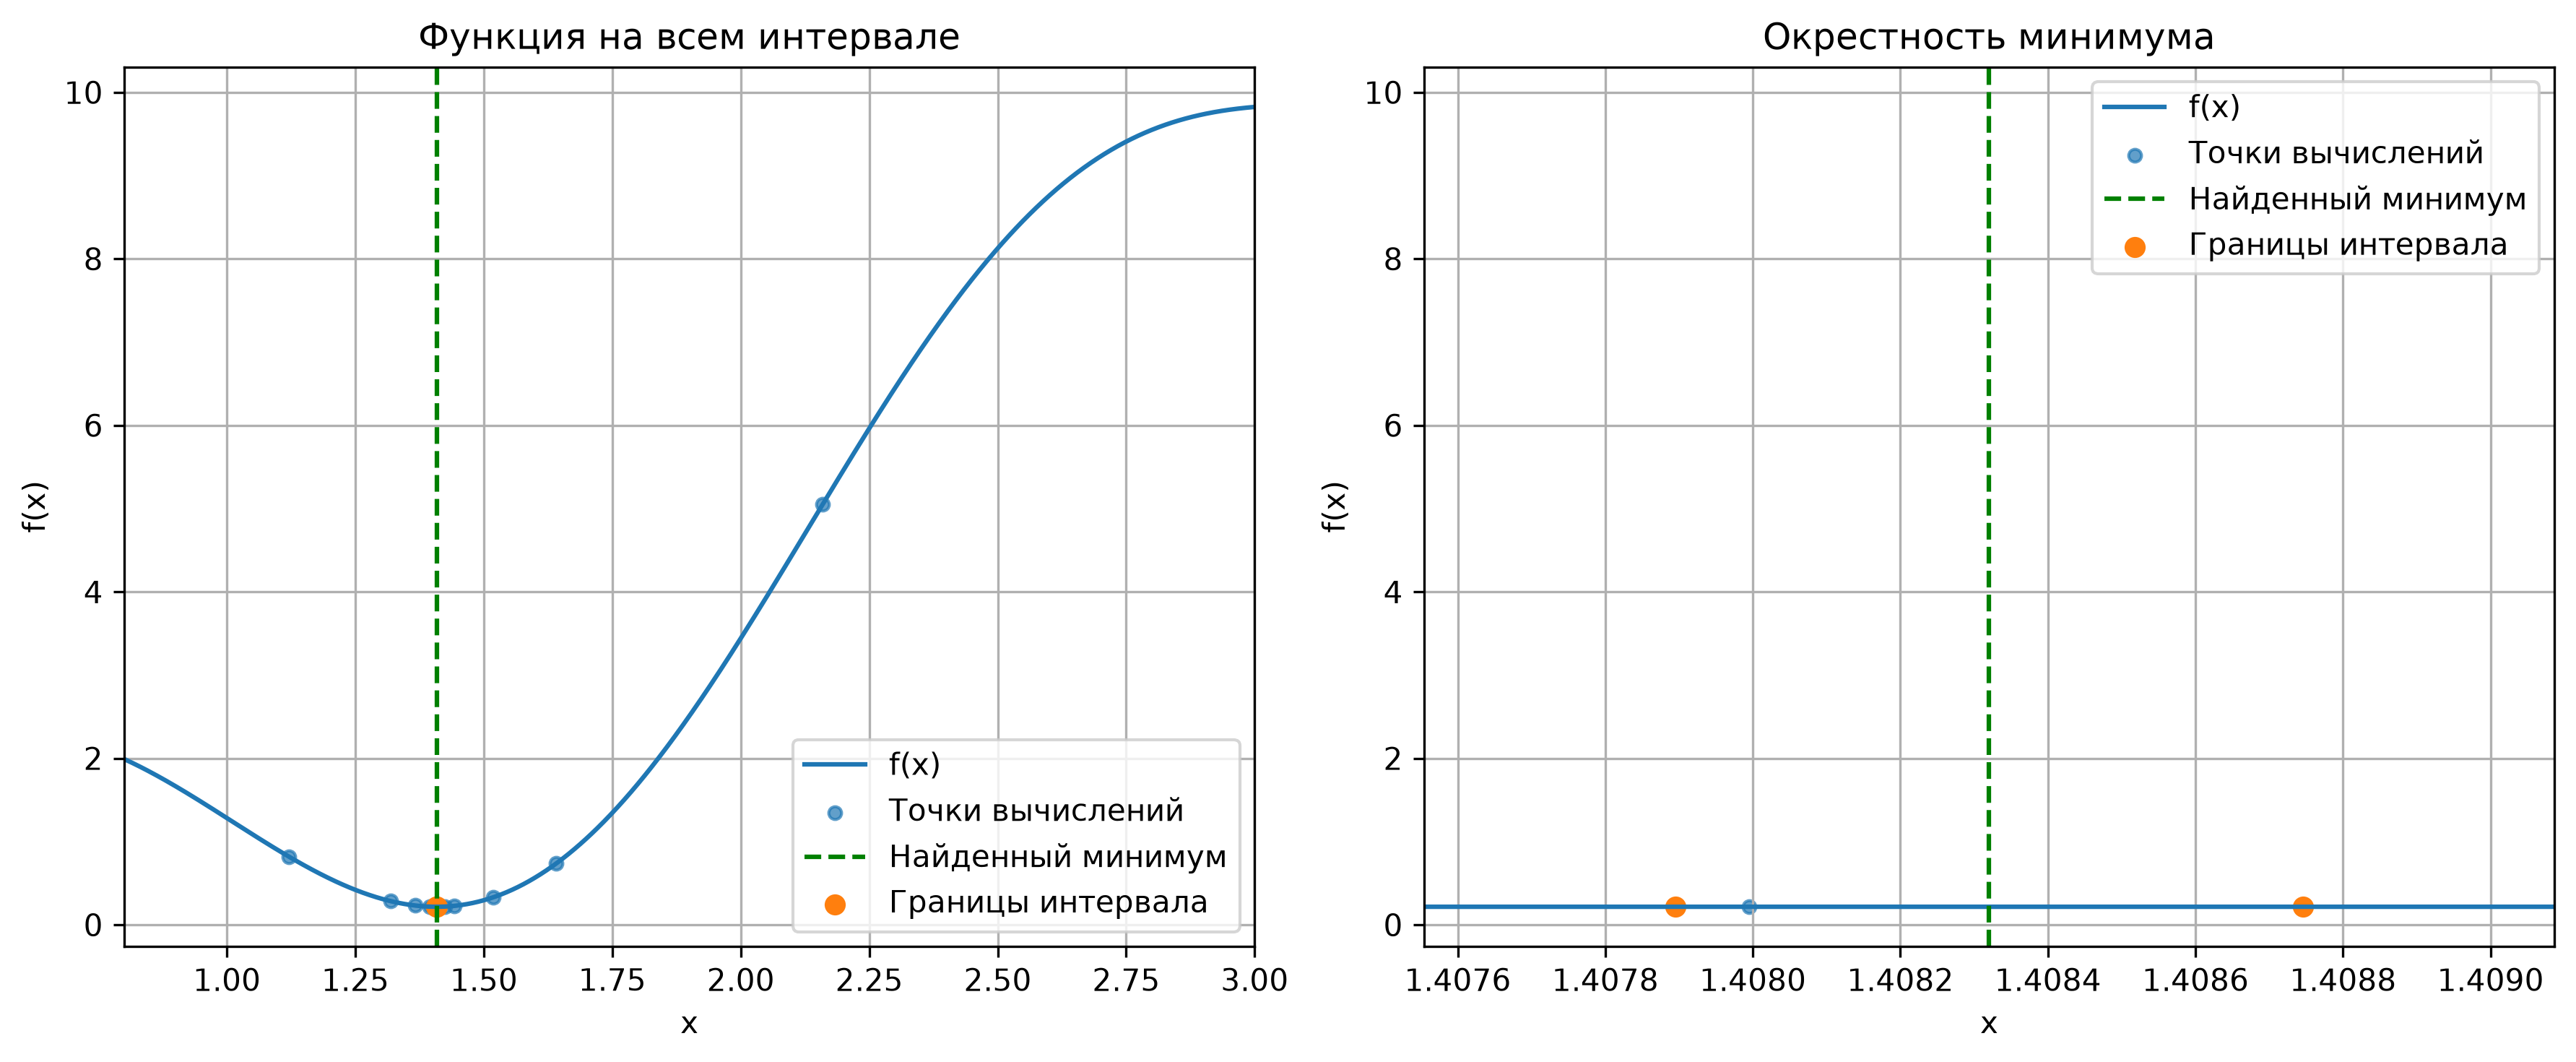
\includegraphics[width=0.95\textwidth]{results/fibonacci/f2.png}
	\caption{Метод Фибоначчи на функции $f_2$.}
	\label{fig:fibonacci-f2}
\end{figure}

\begin{figure}[H]
	\centering
	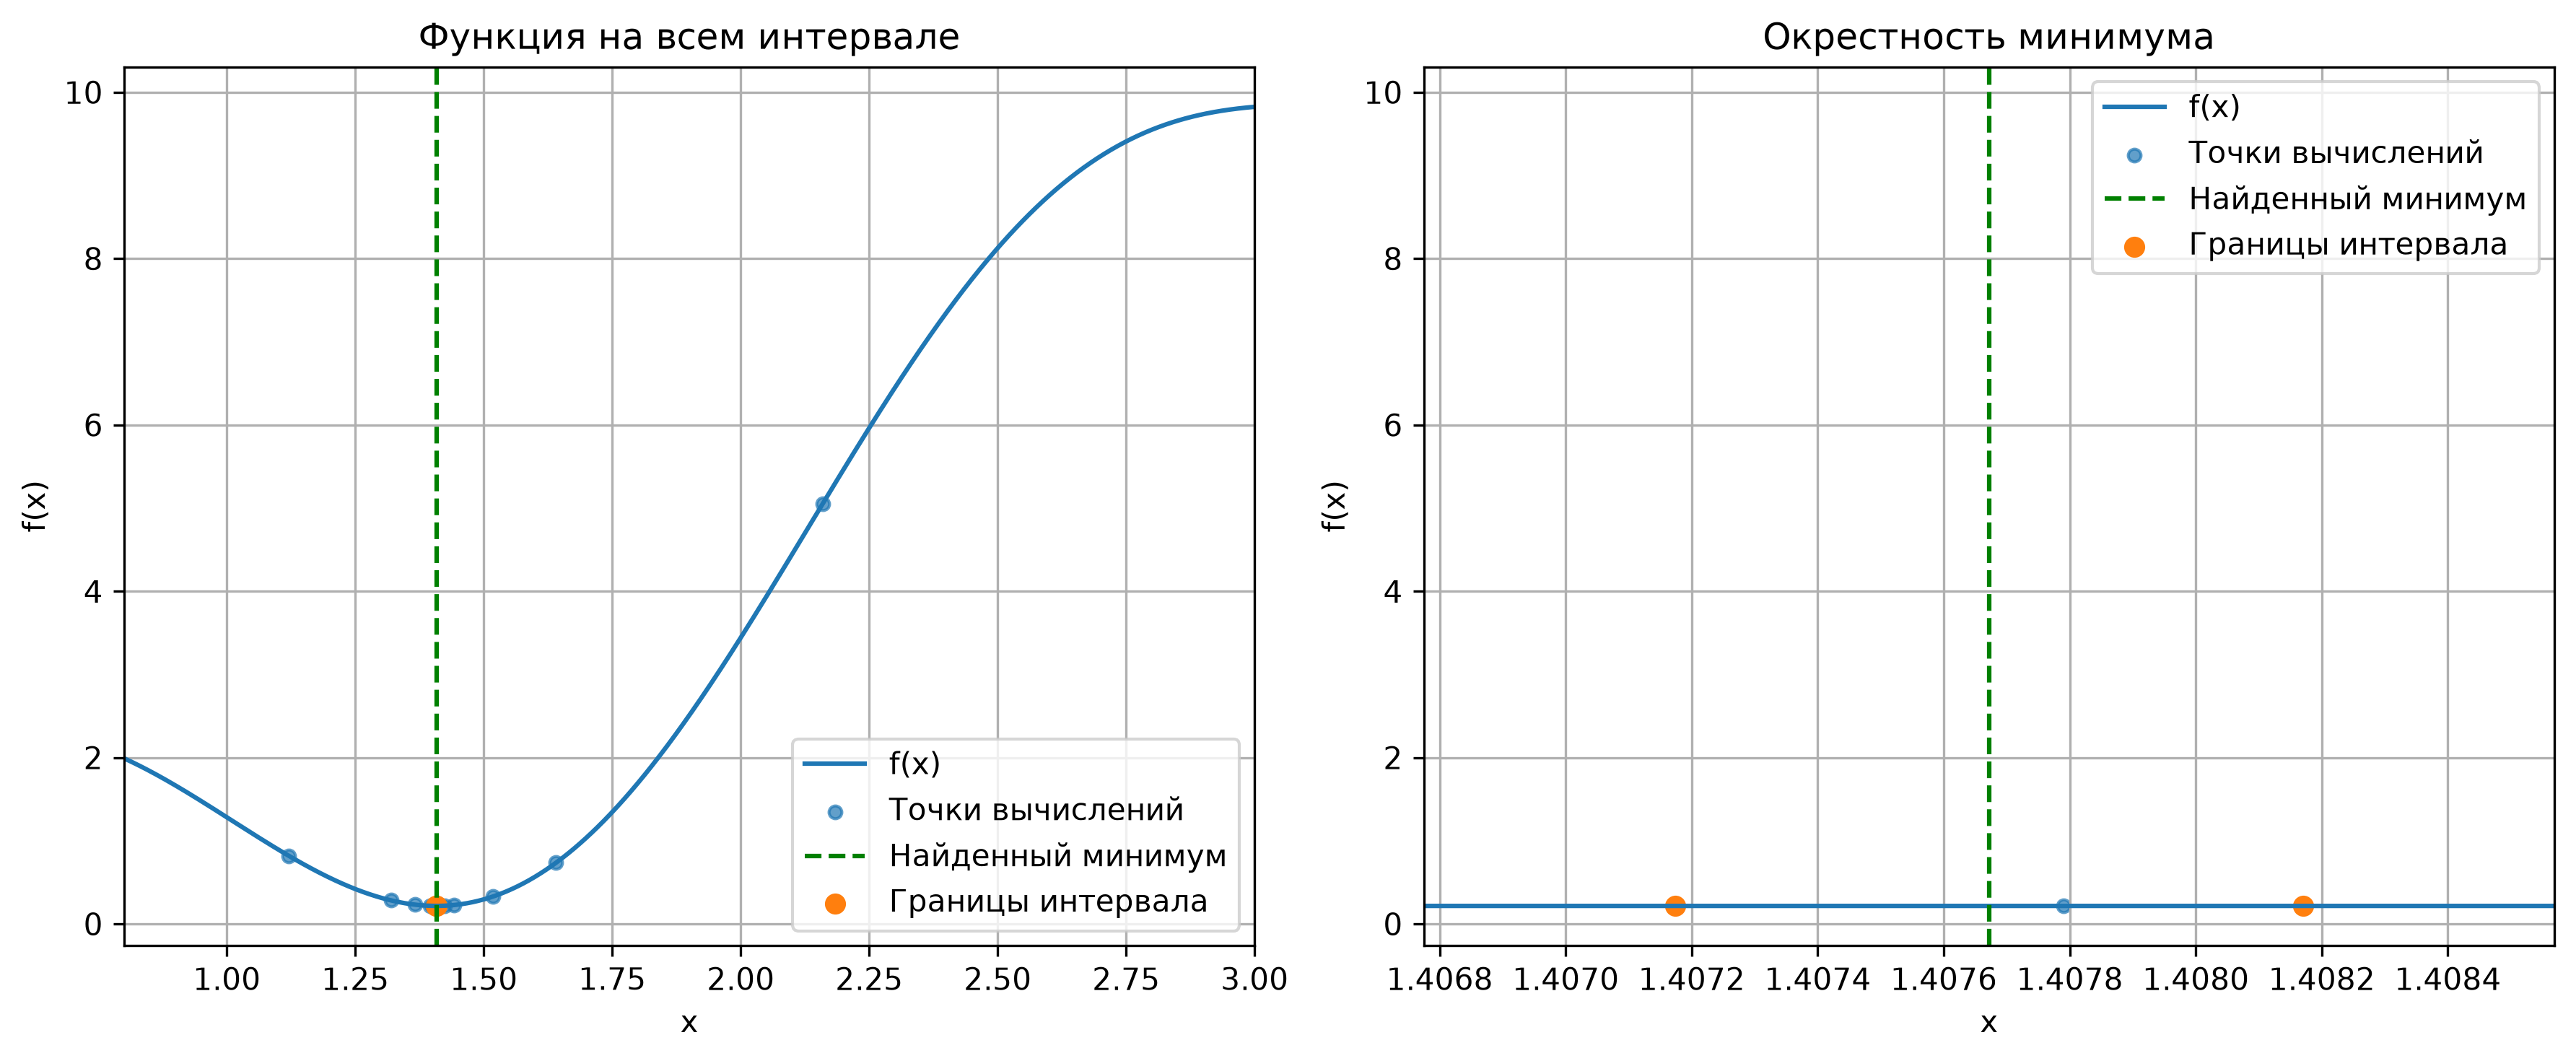
\includegraphics[width=0.95\textwidth]{results/golden_ratio/f2.png}
	\caption{Метод золотого сечения на функции $f_2$.}
	\label{fig:golden-f2}
\end{figure}

\begin{figure}[H]
	\centering
	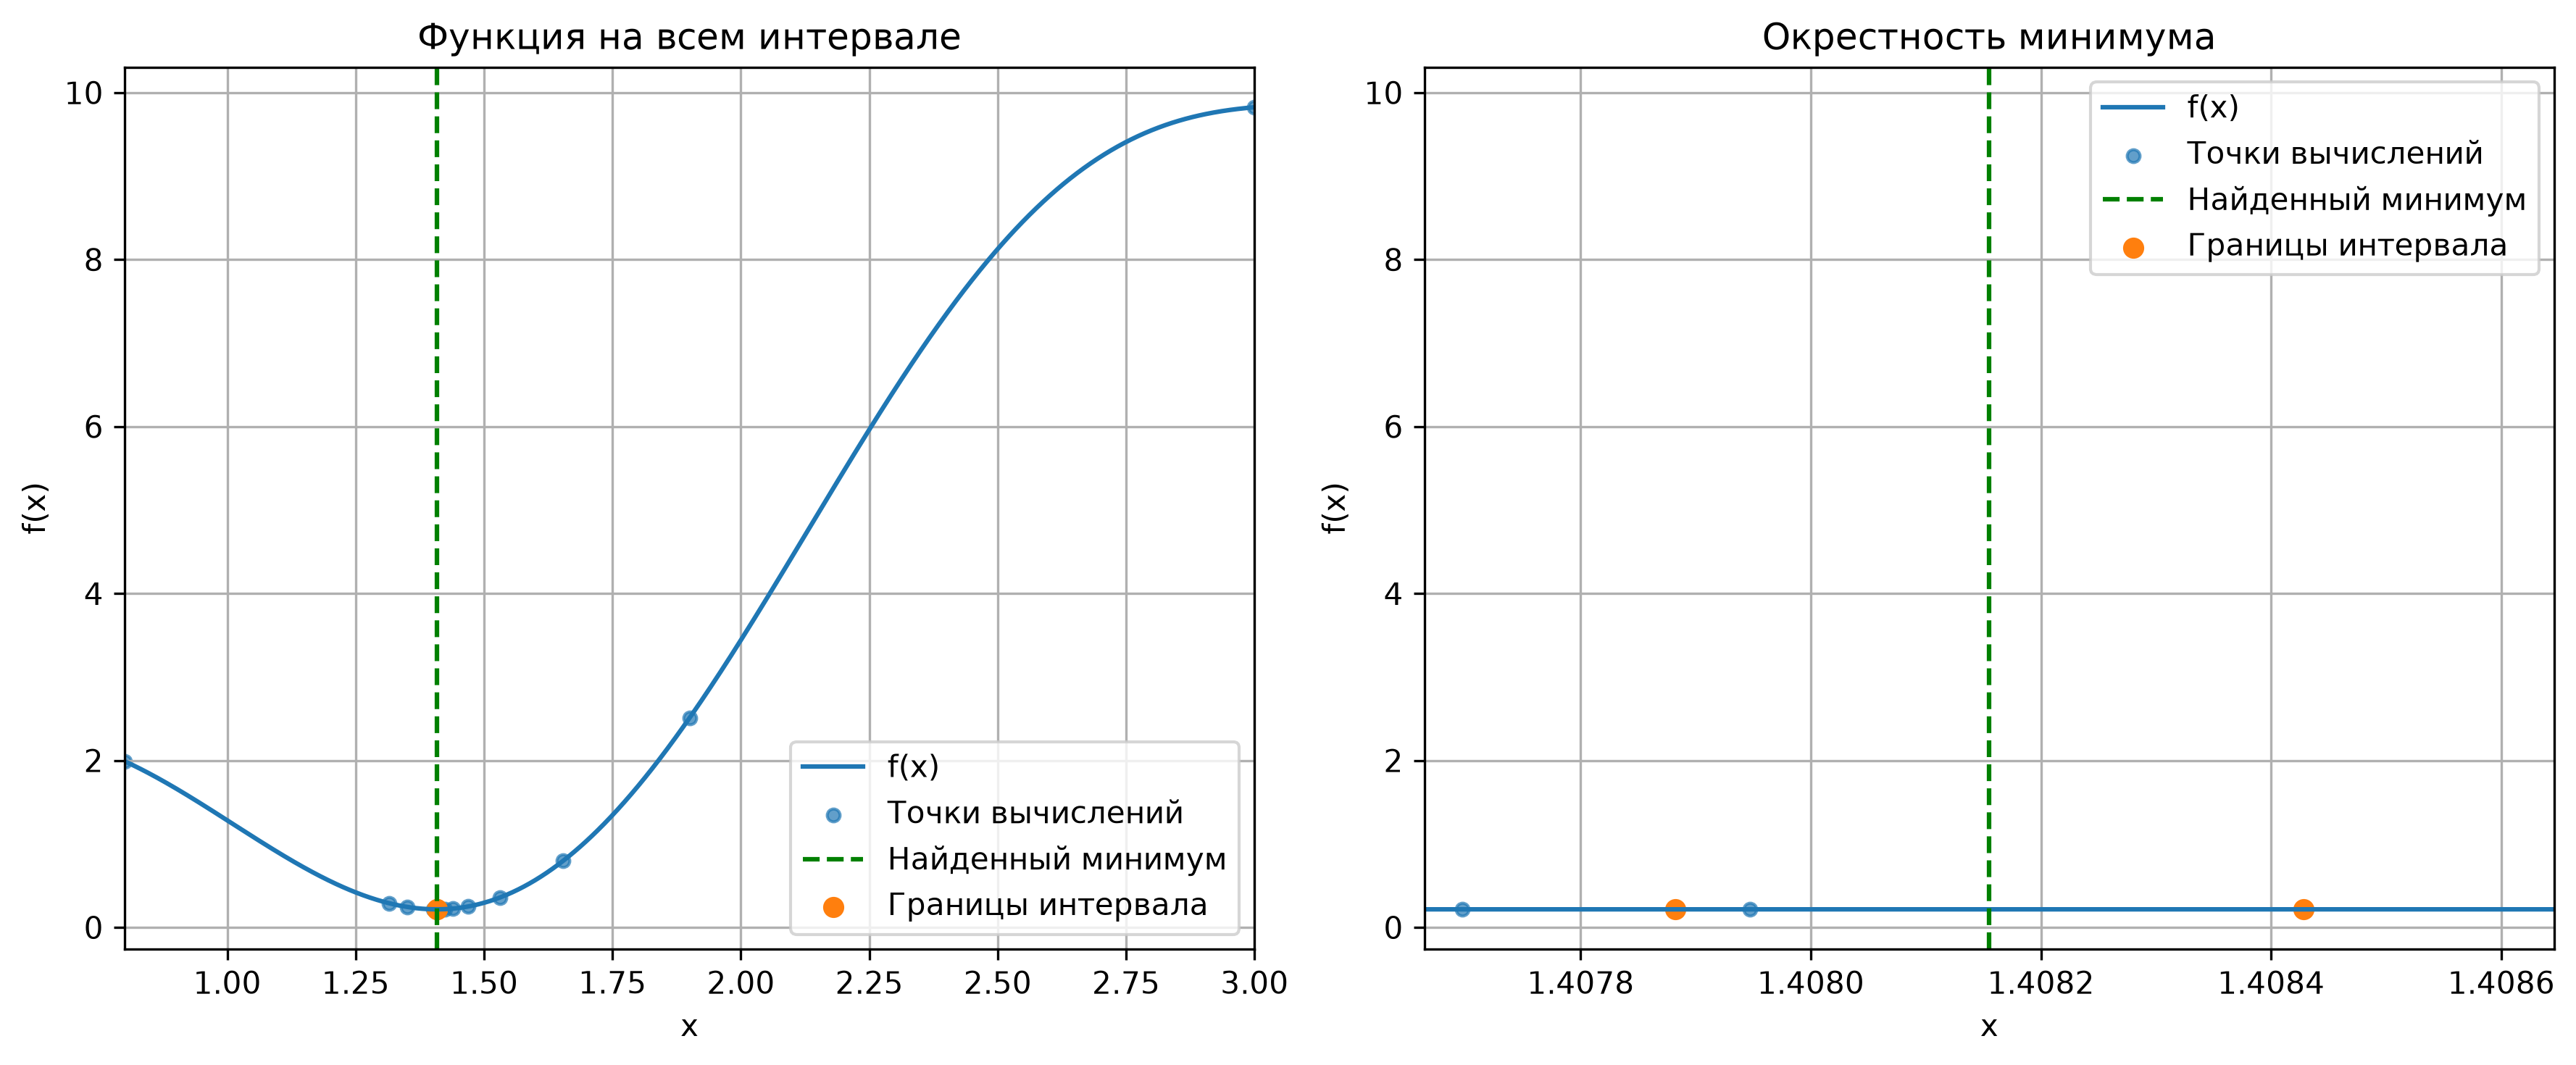
\includegraphics[width=0.95\textwidth]{results/parabola/f2.png}
	\caption{Метод парабол на функции $f_2$.}
	\label{fig:parabola-f2}
\end{figure}

Функция $f_2$ имеет более сложный рельеф из-за синусоидальной составляющей.
Тем не менее на выбранном интервале она сохраняет унимодальное поведение,
поэтому локальные методы сходятся к одному и тому же минимуму. Полученные
графики подтверждают, что уменьшение числа вычислений достигается за счет
повторного использования уже вычисленных внутренних точек.

\subsection{Скорость сходимости локальных методов}

На рисунках~\ref{fig:convergence-f1} и~\ref{fig:convergence-f2} по вертикальной
оси отложена длина текущего отрезка локализации в логарифмическом масштабе,
а по горизонтальной --- число вычислений функции. Такое представление позволяет
сравнивать методы с разными законами сходимости на одной диаграмме.

\begin{figure}[H]
	\centering
	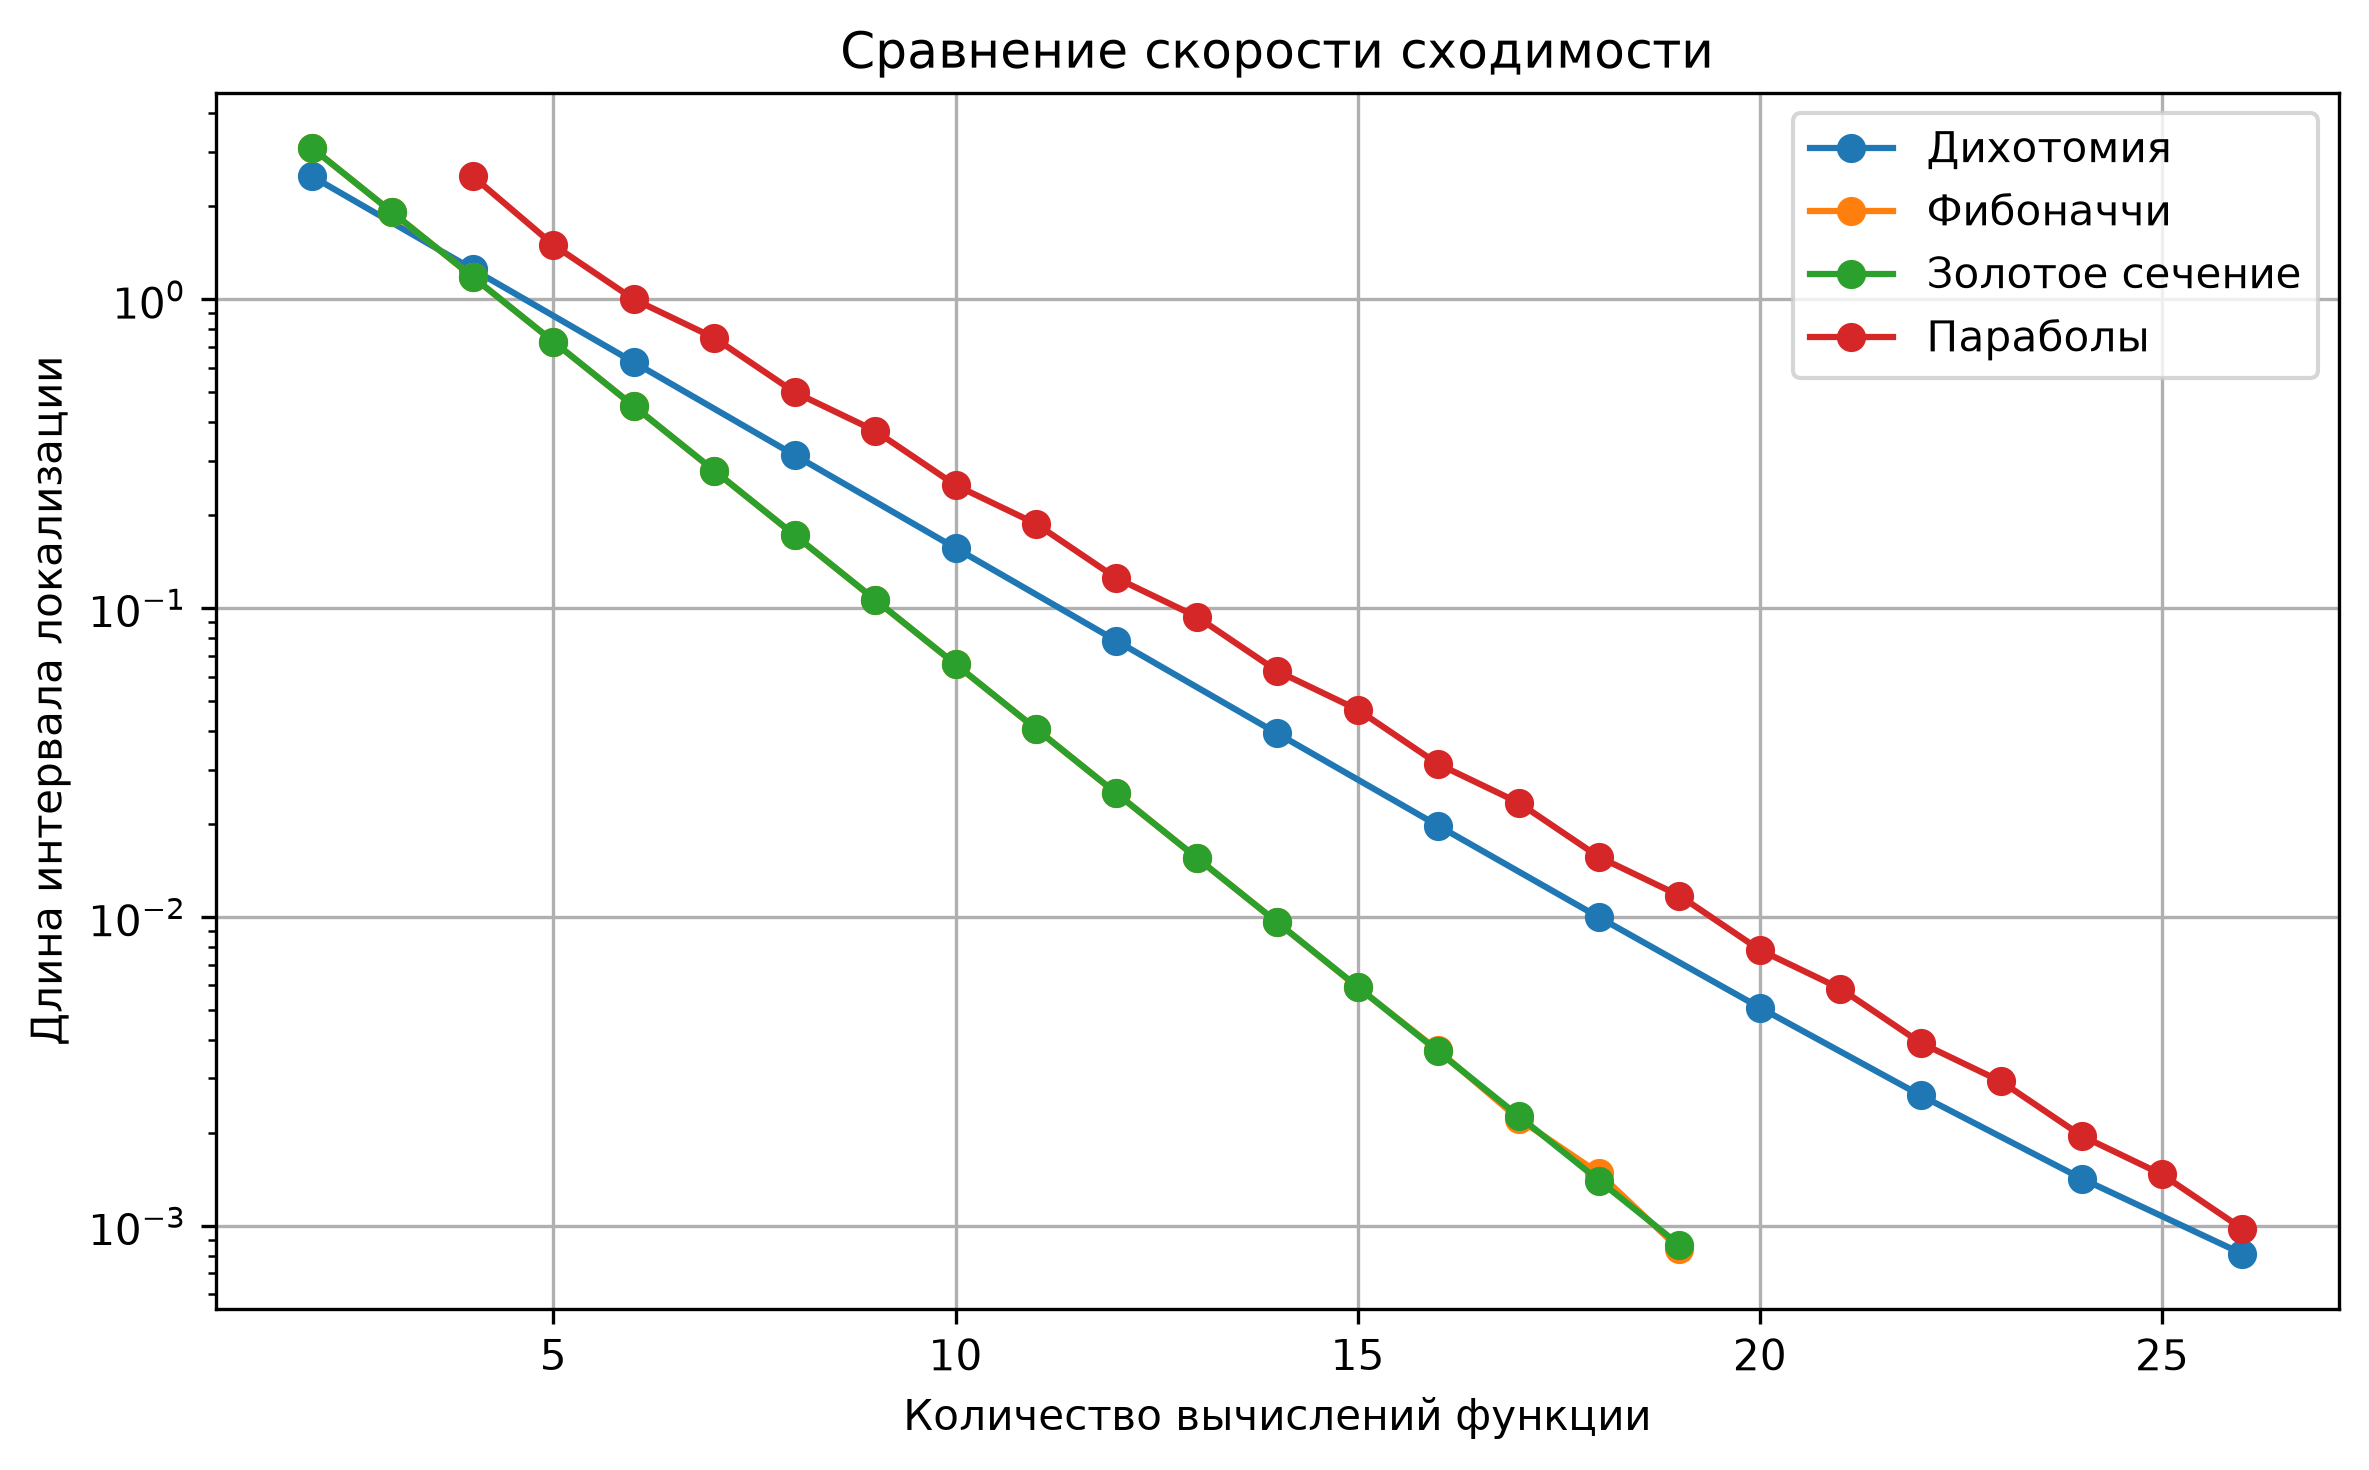
\includegraphics[width=0.95\textwidth]{results/convergence/comparison_f1.png}
	\caption{Скорость сходимости локальных методов на функции $f_1$.}
	\label{fig:convergence-f1}
\end{figure}

\begin{figure}[H]
	\centering
	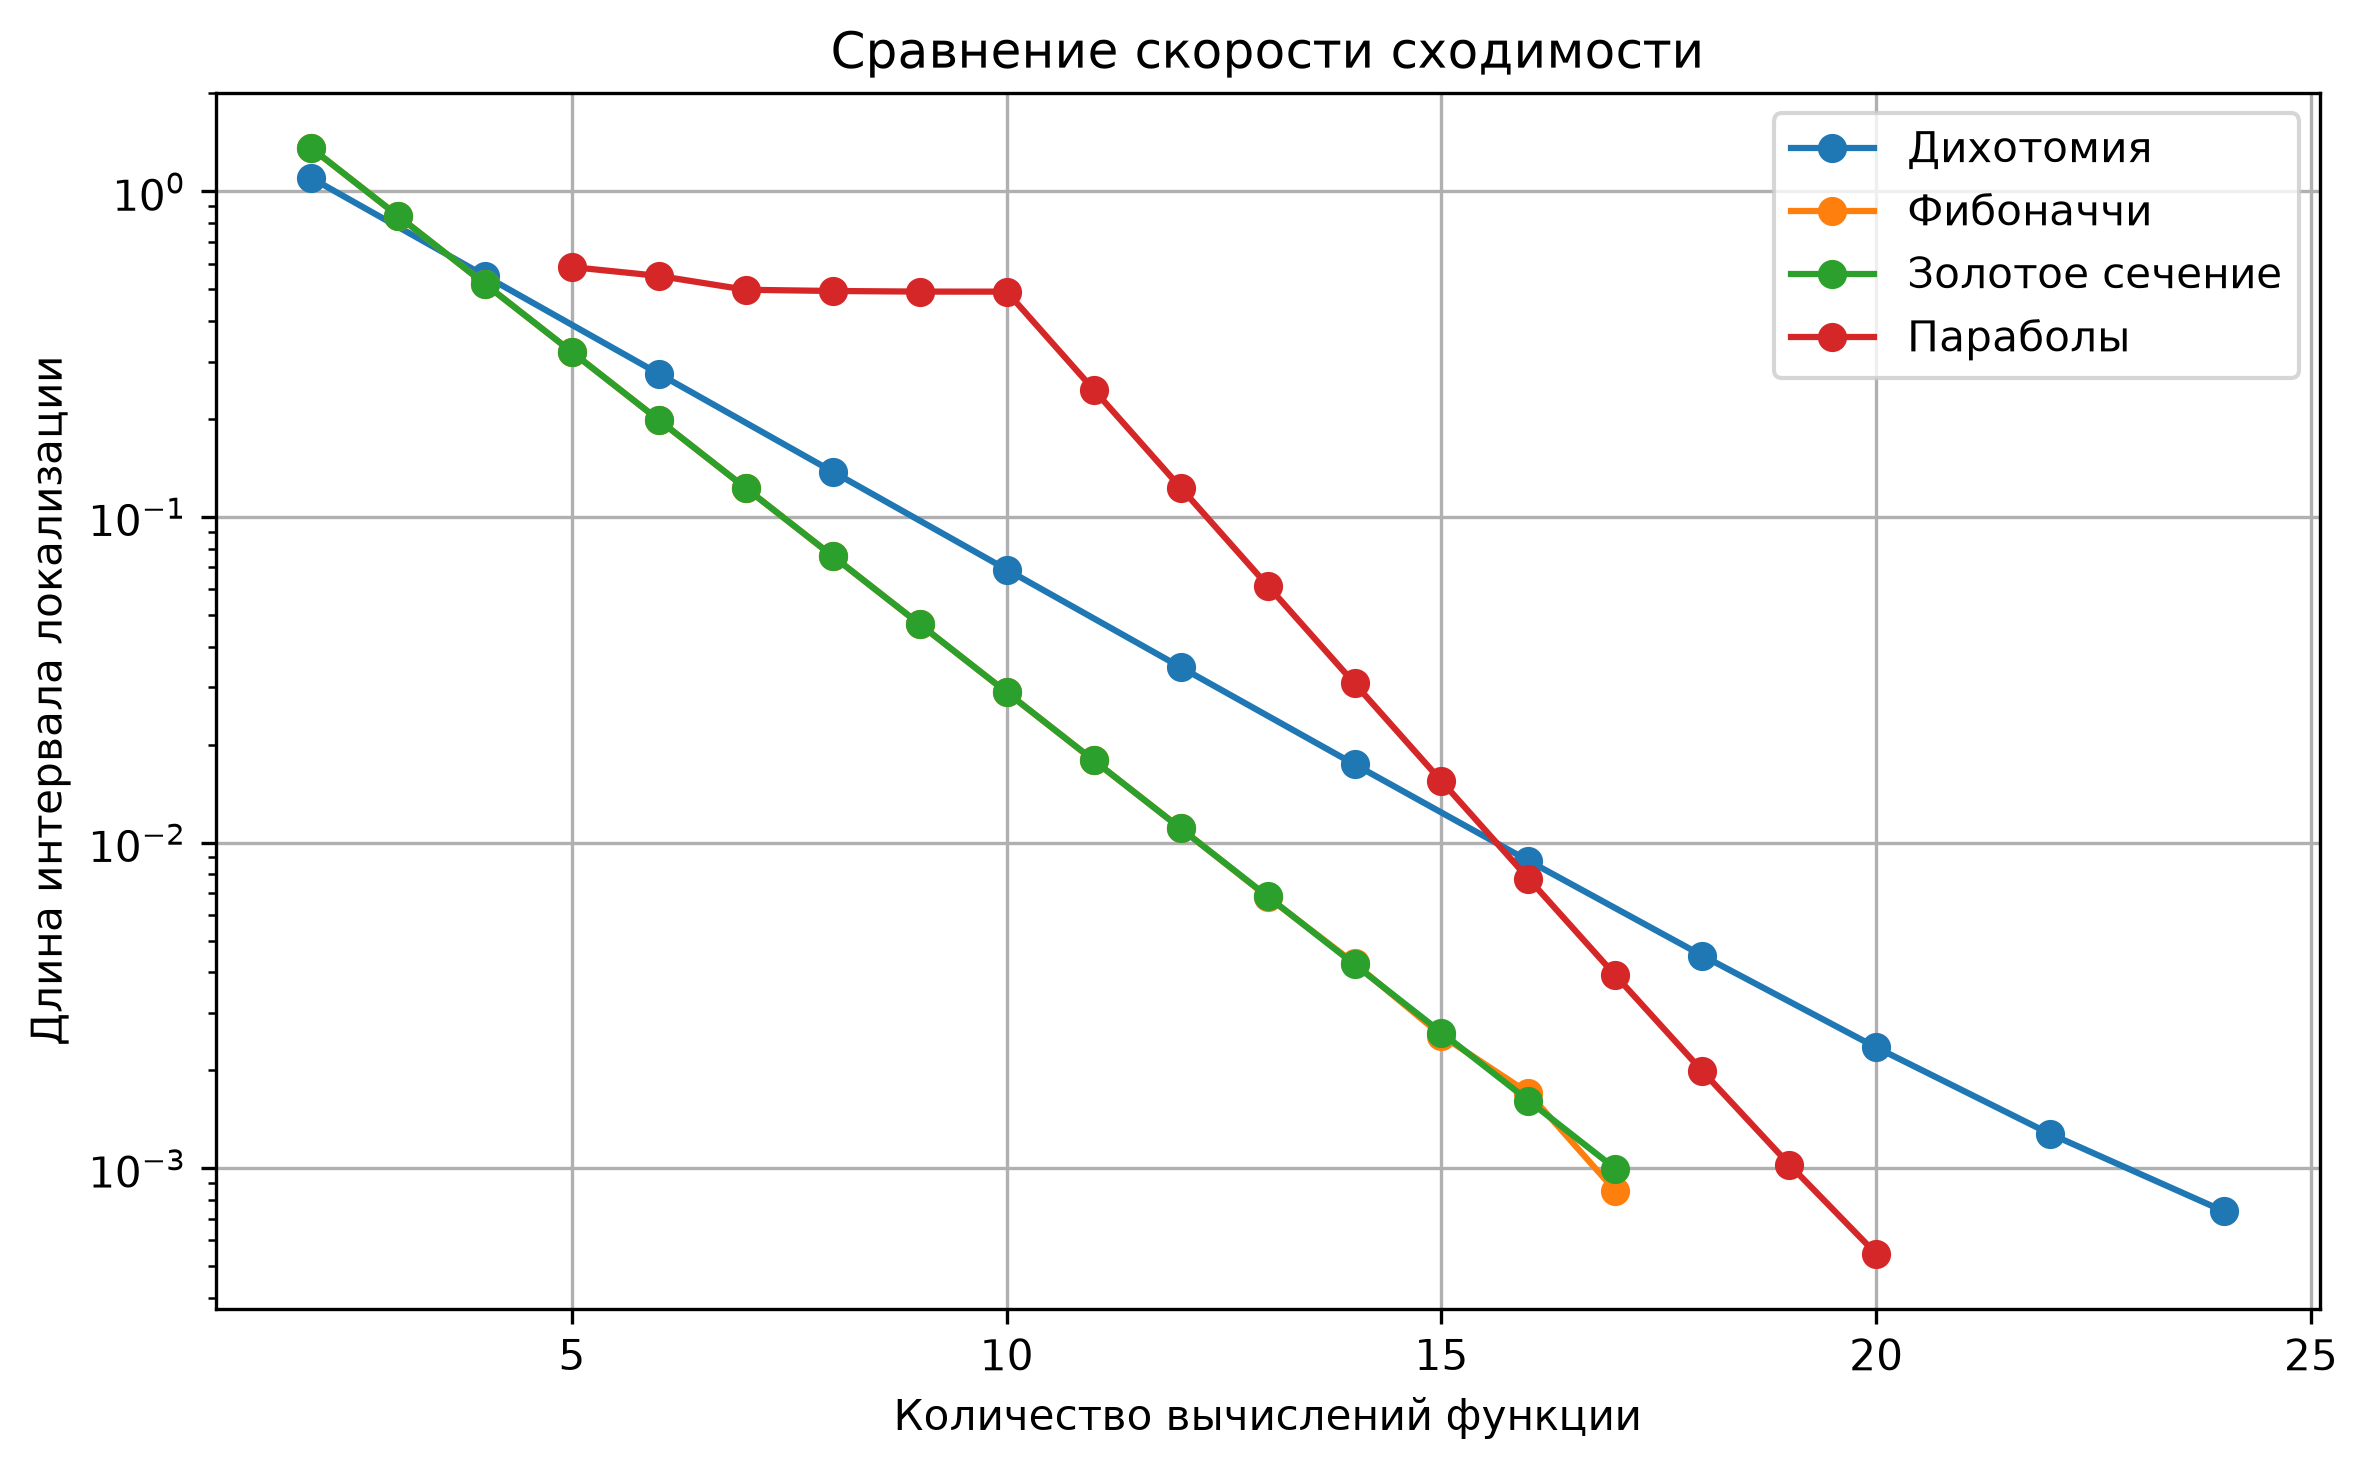
\includegraphics[width=0.95\textwidth]{results/convergence/comparison_f2.png}
	\caption{Скорость сходимости локальных методов на функции $f_2$.}
	\label{fig:convergence-f2}
\end{figure}

По графикам видно, что методы Фибоначчи и золотого сечения обеспечивают
устойчивое уменьшение длины интервала при малом числе вычислений. Метод парабол
может сходиться быстрее на гладких участках функции, однако его эффективность
зависит от качества квадратичной аппроксимации. Пассивный поиск не строит
итерационную последовательность локализации и поэтому на графике сходимости
не представлен.

\subsection{Глобальные методы}

Для мультимодальной функции $f_3$ применялись равномерный перебор и метод
ломаных. Результаты равномерного перебора и метода ломаных показаны на
рисунках~\ref{fig:search-f3} и~\ref{fig:broken-lines-f3} соответственно.
\begin{figure}[H]
	\centering
	
\includegraphics[width=0.95\textwidth]{results/search/f3.png}
	\caption{Равномерный перебор на функции $f_3$.}
	\label{fig:search-f3}
\end{figure}

\begin{figure}[H]
	\centering
	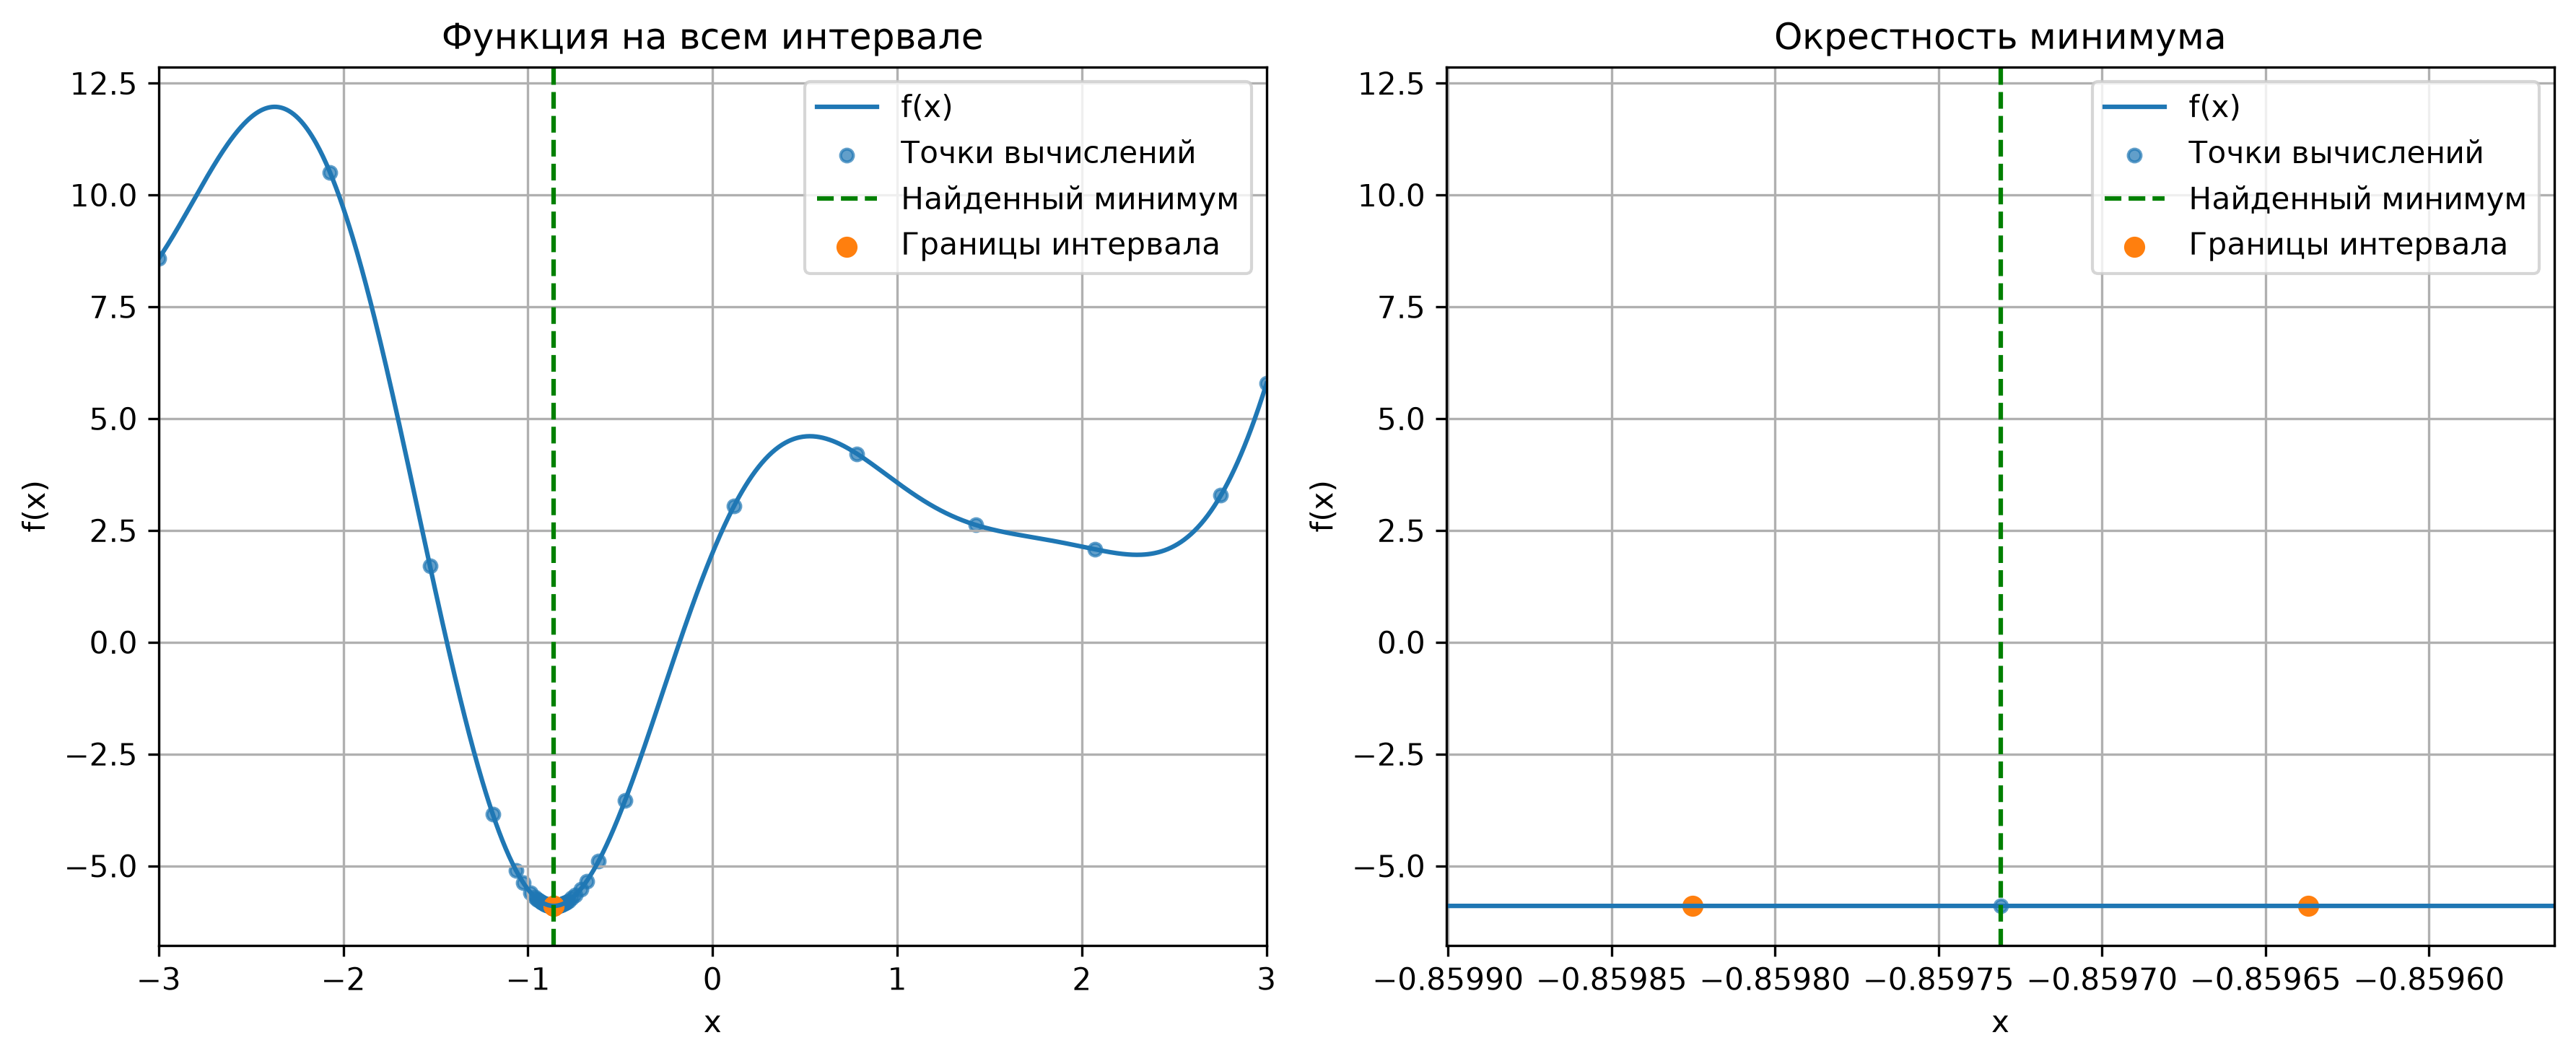
\includegraphics[width=0.95\textwidth]{results/broken_lines/f3.png}
	\caption{Метод ломаных на функции $f_3$.}
	\label{fig:broken-lines-f3}
\end{figure}

Равномерный перебор исследует весь интервал с одинаковым шагом, поэтому его
поведение не зависит от локальной структуры функции. Метод ломаных распределяет
новые вычисления адаптивно: больше точек появляется в интервалах, которые имеют
наиболее перспективную нижнюю оценку. Это позволяет использовать информацию
о константе Липшица и уточнять область глобального минимума.

\subsection{Сравнение при одинаковом числе вычислений}

Для корректного сравнения глобальных методов им был задан одинаковый бюджет
вычислений функции. На рисунках~\ref{fig:global-x-error} и
~\ref{fig:global-f-error} показаны ошибки координаты минимума и значения
функции относительно эталонного решения, полученного на плотной сетке.

\begin{figure}[H]
	\centering
	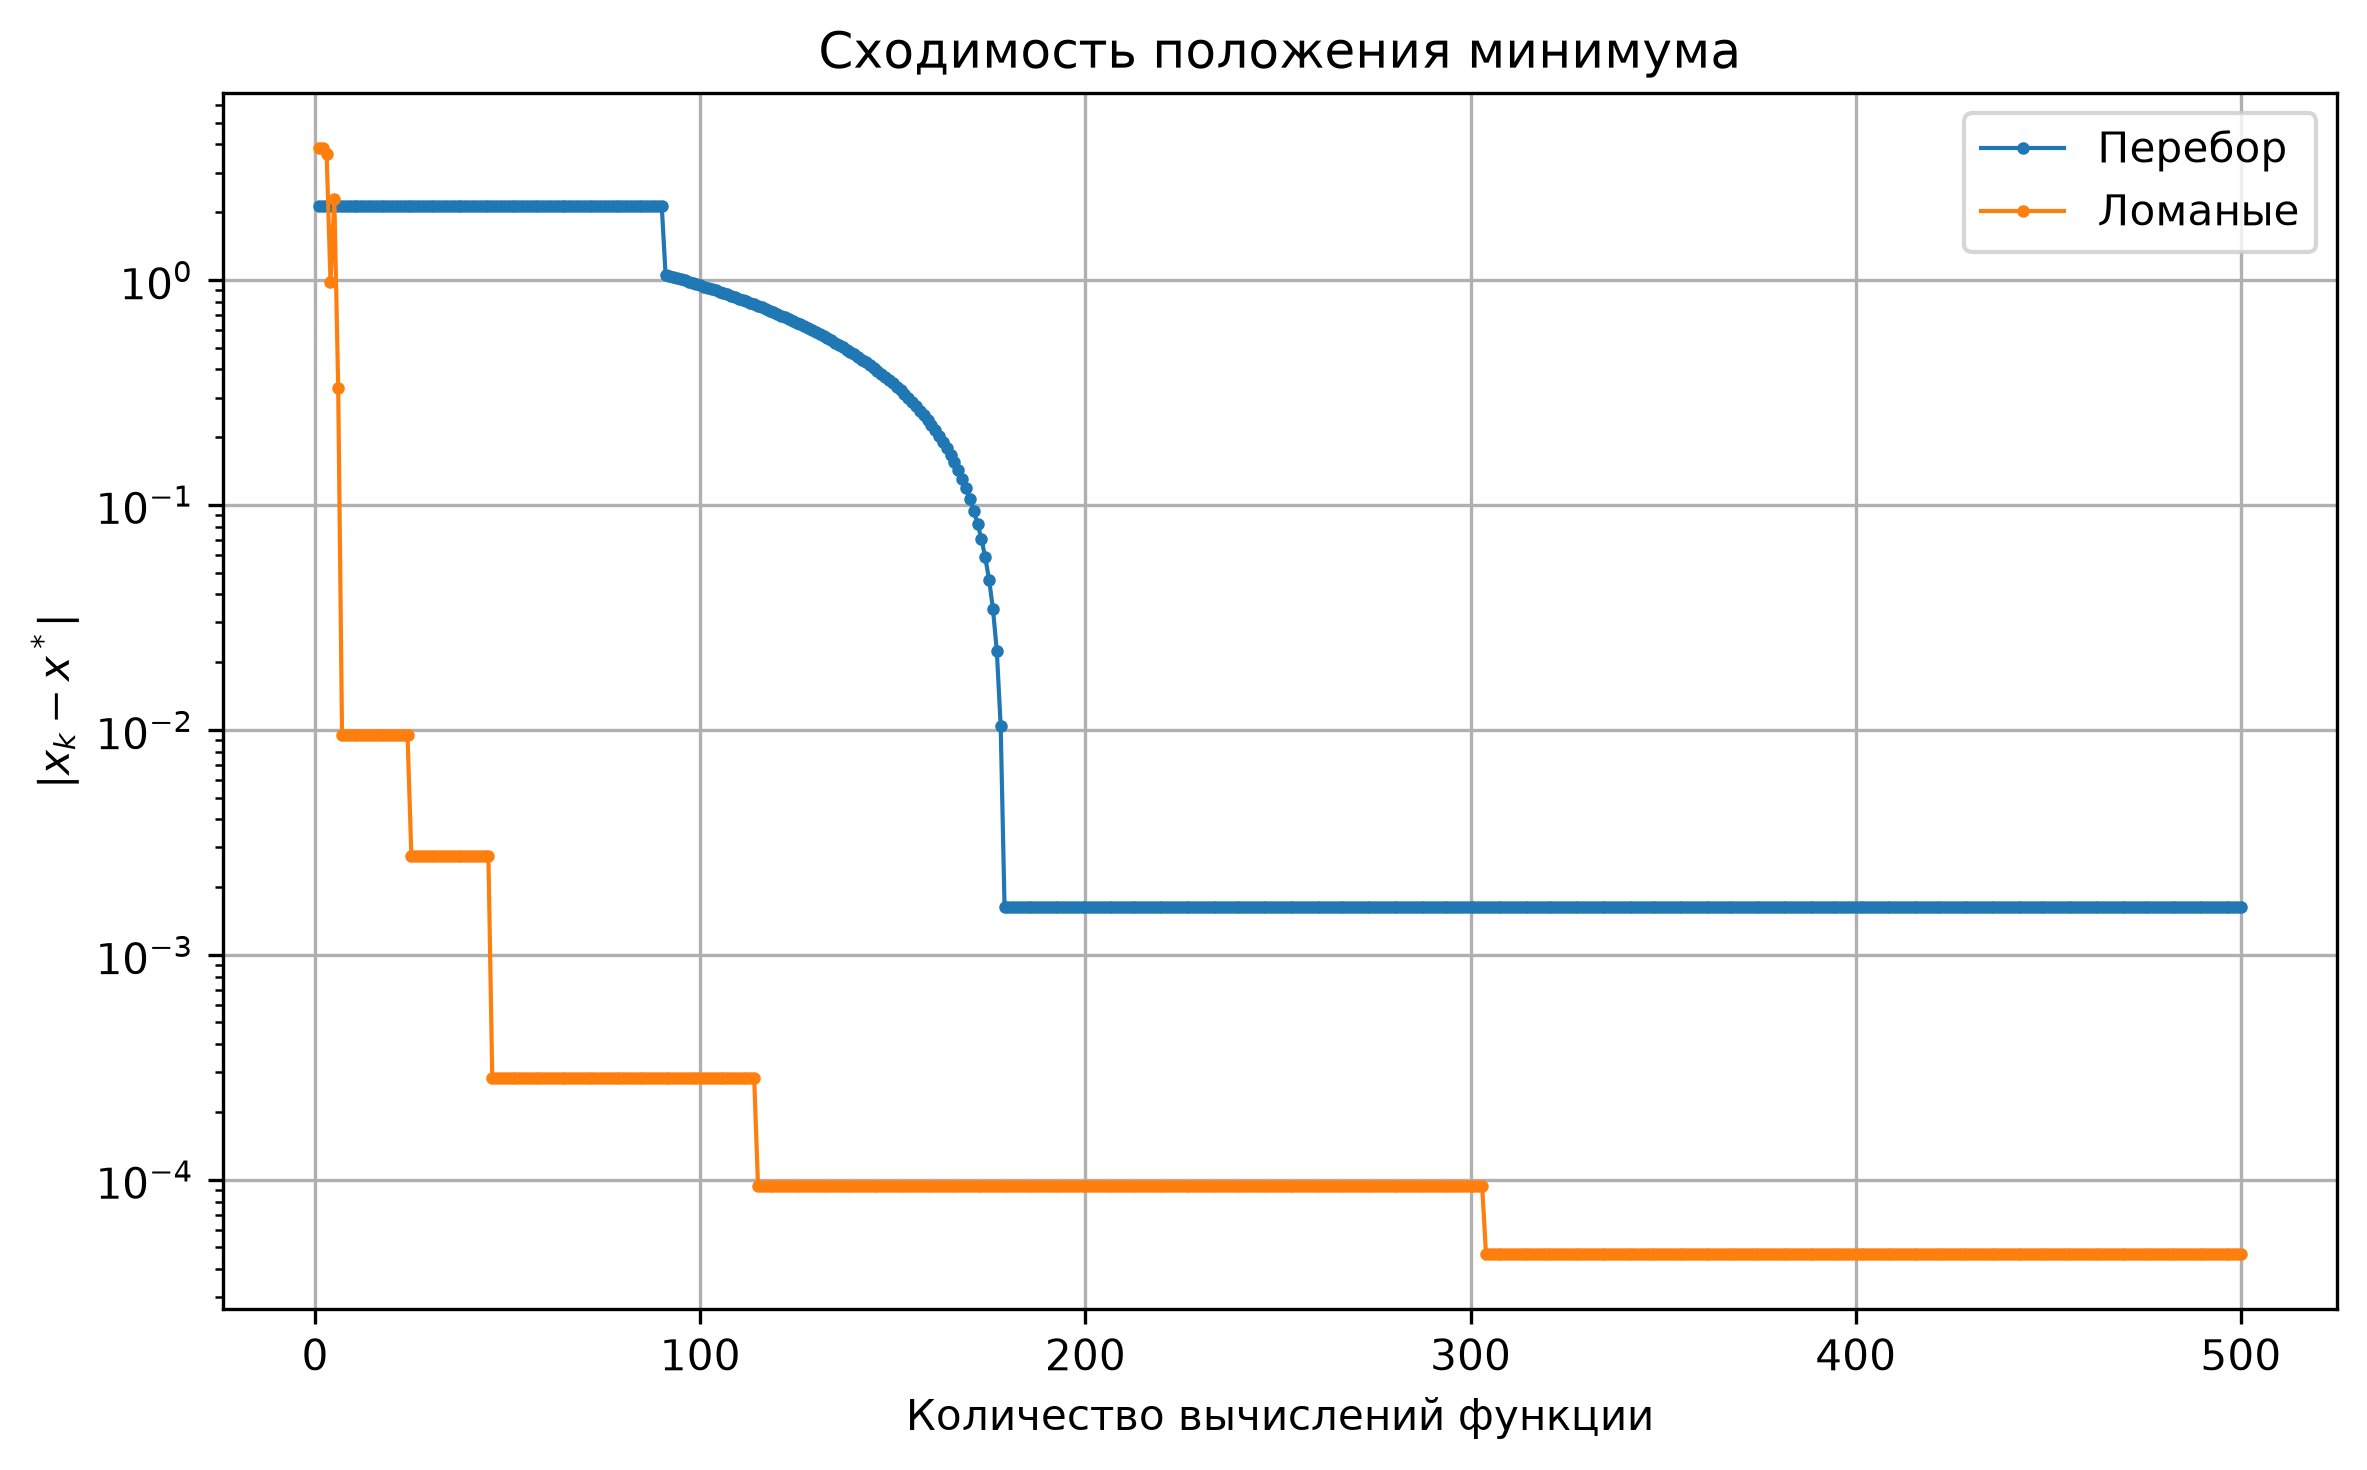
\includegraphics[width=0.88\textwidth]{results/comparison/global_x_convergence_f3.png}
	\caption{Ошибка координаты минимума при одинаковом числе вычислений.}
	\label{fig:global-x-error}
\end{figure}

\begin{figure}[H]
	\centering
	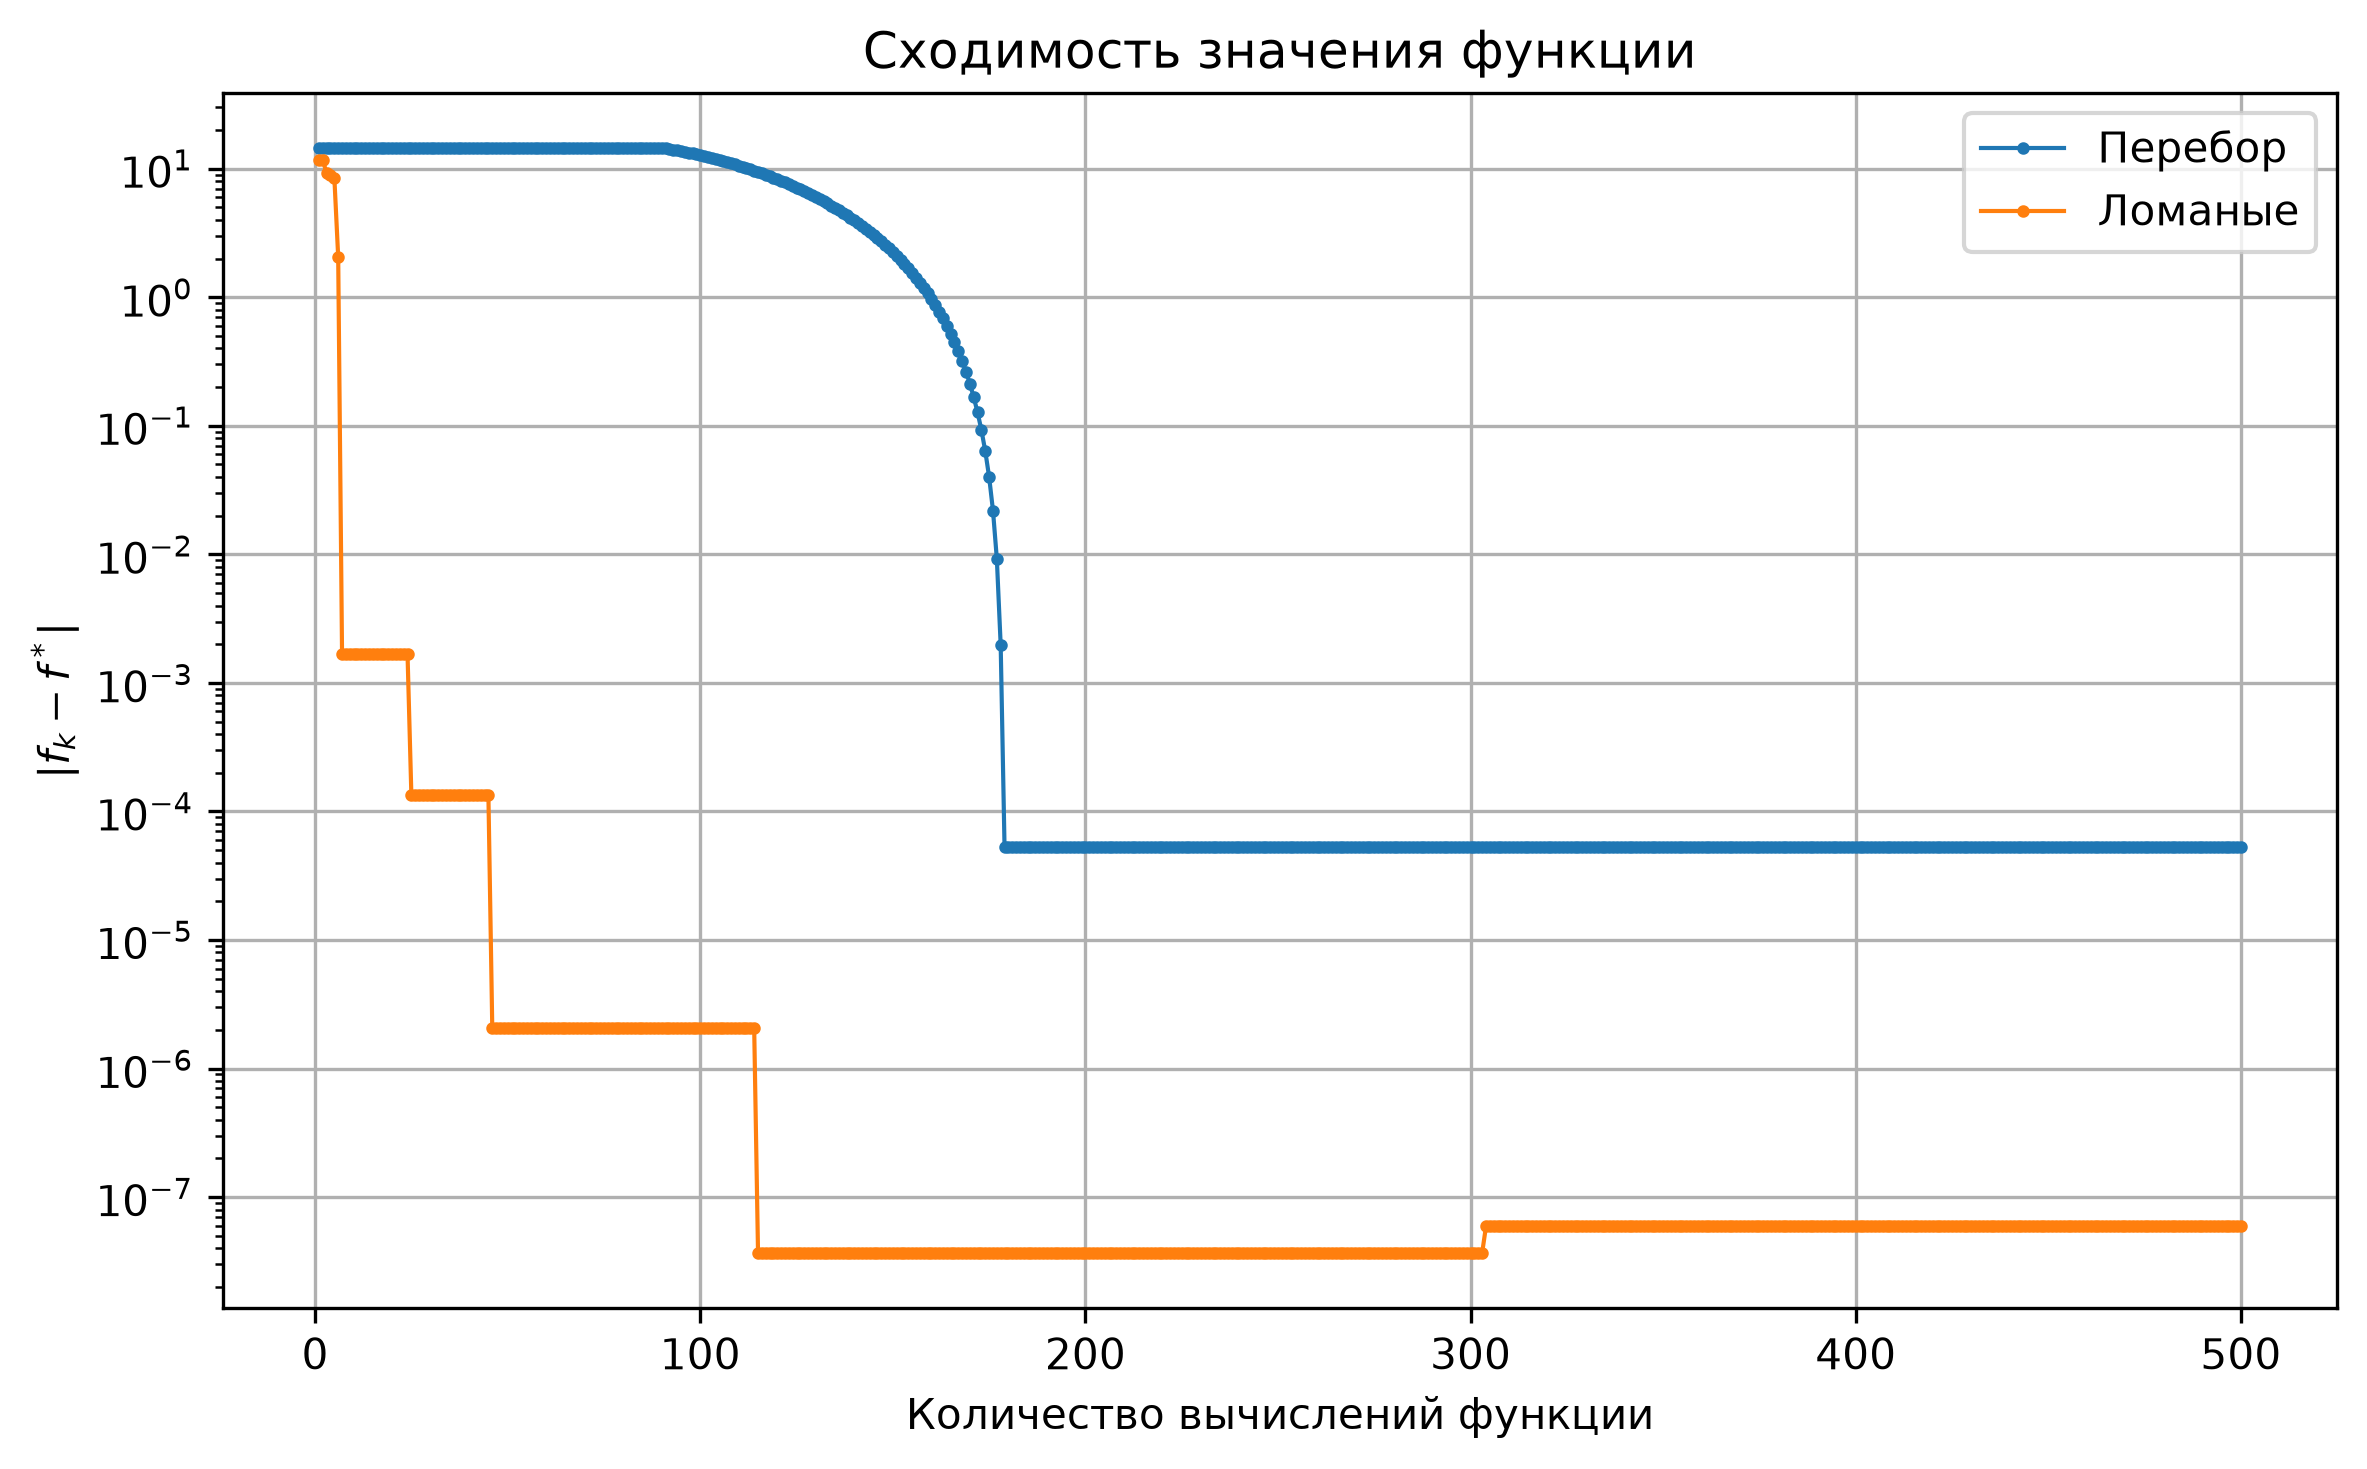
\includegraphics[width=0.88\textwidth]{results/comparison/global_f_convergence_f3.png}
	\caption{Ошибка значения функции при одинаковом числе вычислений.}
	\label{fig:global-f-error}
\end{figure}

Эти графики показывают, что метод ломаных обеспечивает более точное
приближение глобального минимума по сравнению с равномерным перебором 
при одинаковом числе вычислений функции. Метод перебора требует значительно
большего числа вычислений для достижения сопоставимой точности и выходит
быстро выходит на плато из-за ограниченной ширины равномерной сетки.

\newpage

Отдельно выполнено сравнение локальных методов при одинаковом числе вычислений.
Результат представлен на рисунках~\ref{fig:local-comparison-f1} и~\ref{fig:local-comparison-f2}.

\begin{figure}[H]
	\centering
	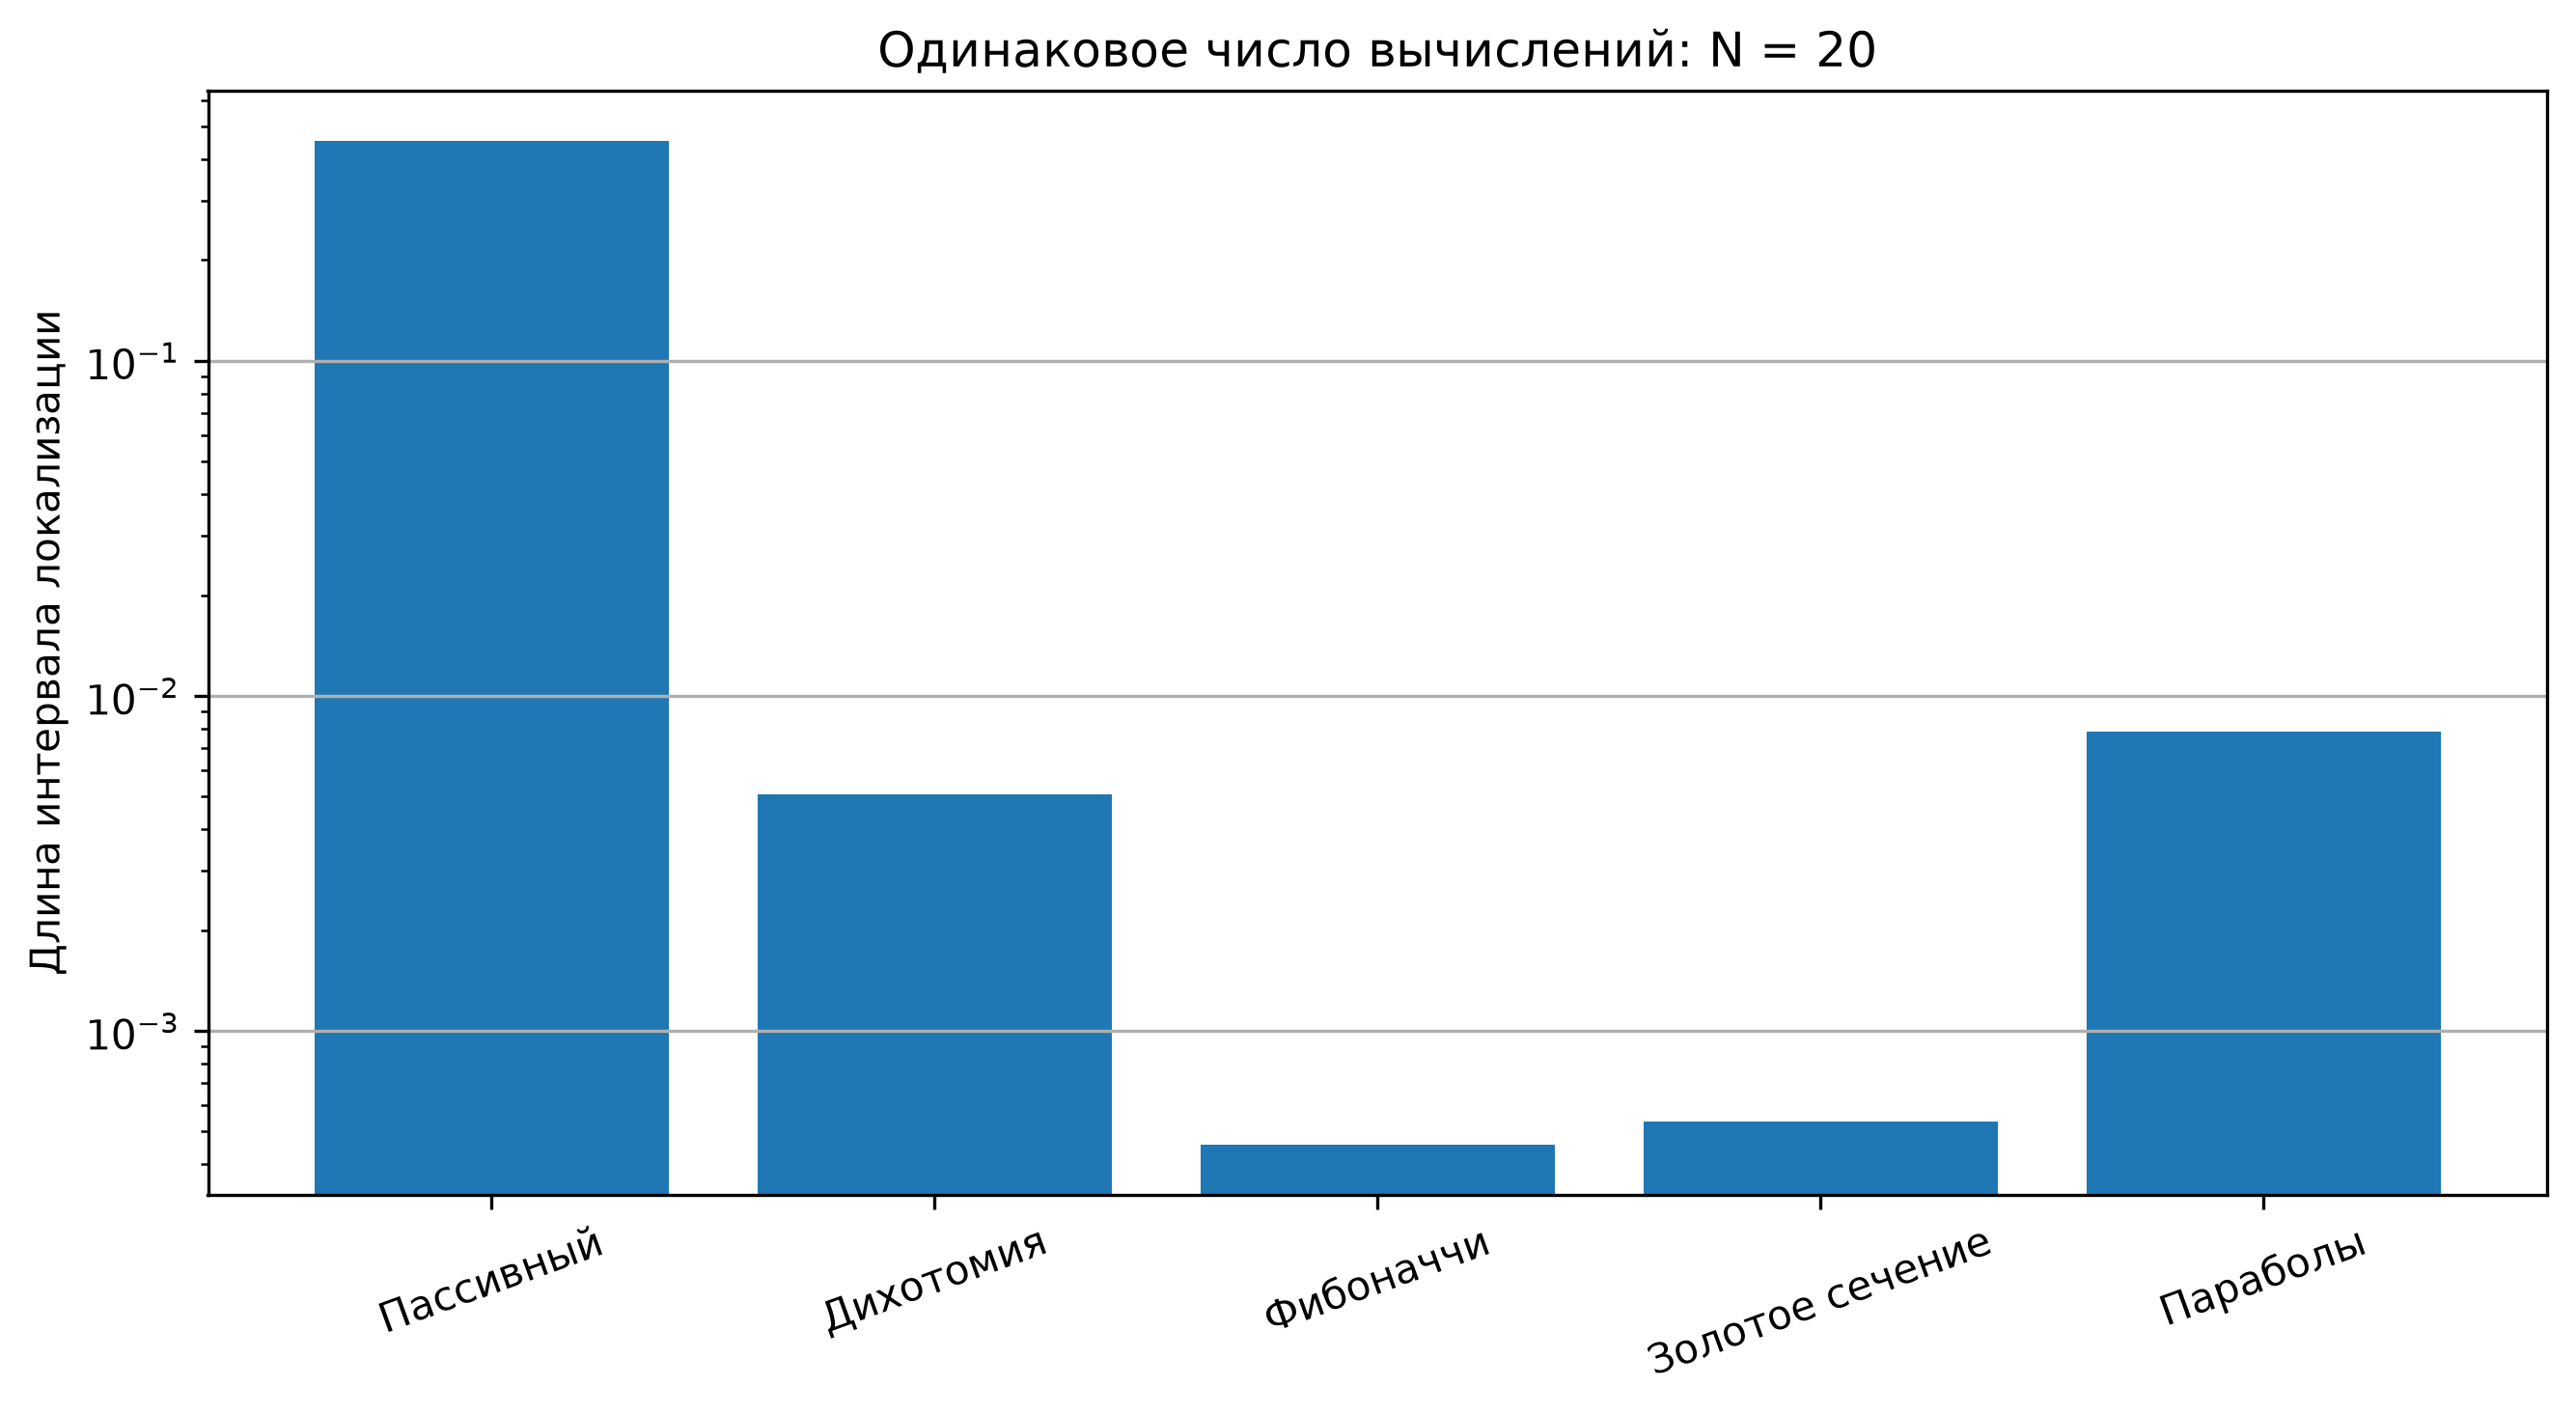
\includegraphics[width=0.88\textwidth]{results/comparison/local_f1.png}
	\caption{Сравнение длины итогового интервала при одинаковом числе вычислений для $f_1$.}
	\label{fig:local-comparison-f1}
\end{figure}

\begin{figure}[H]
	\centering
	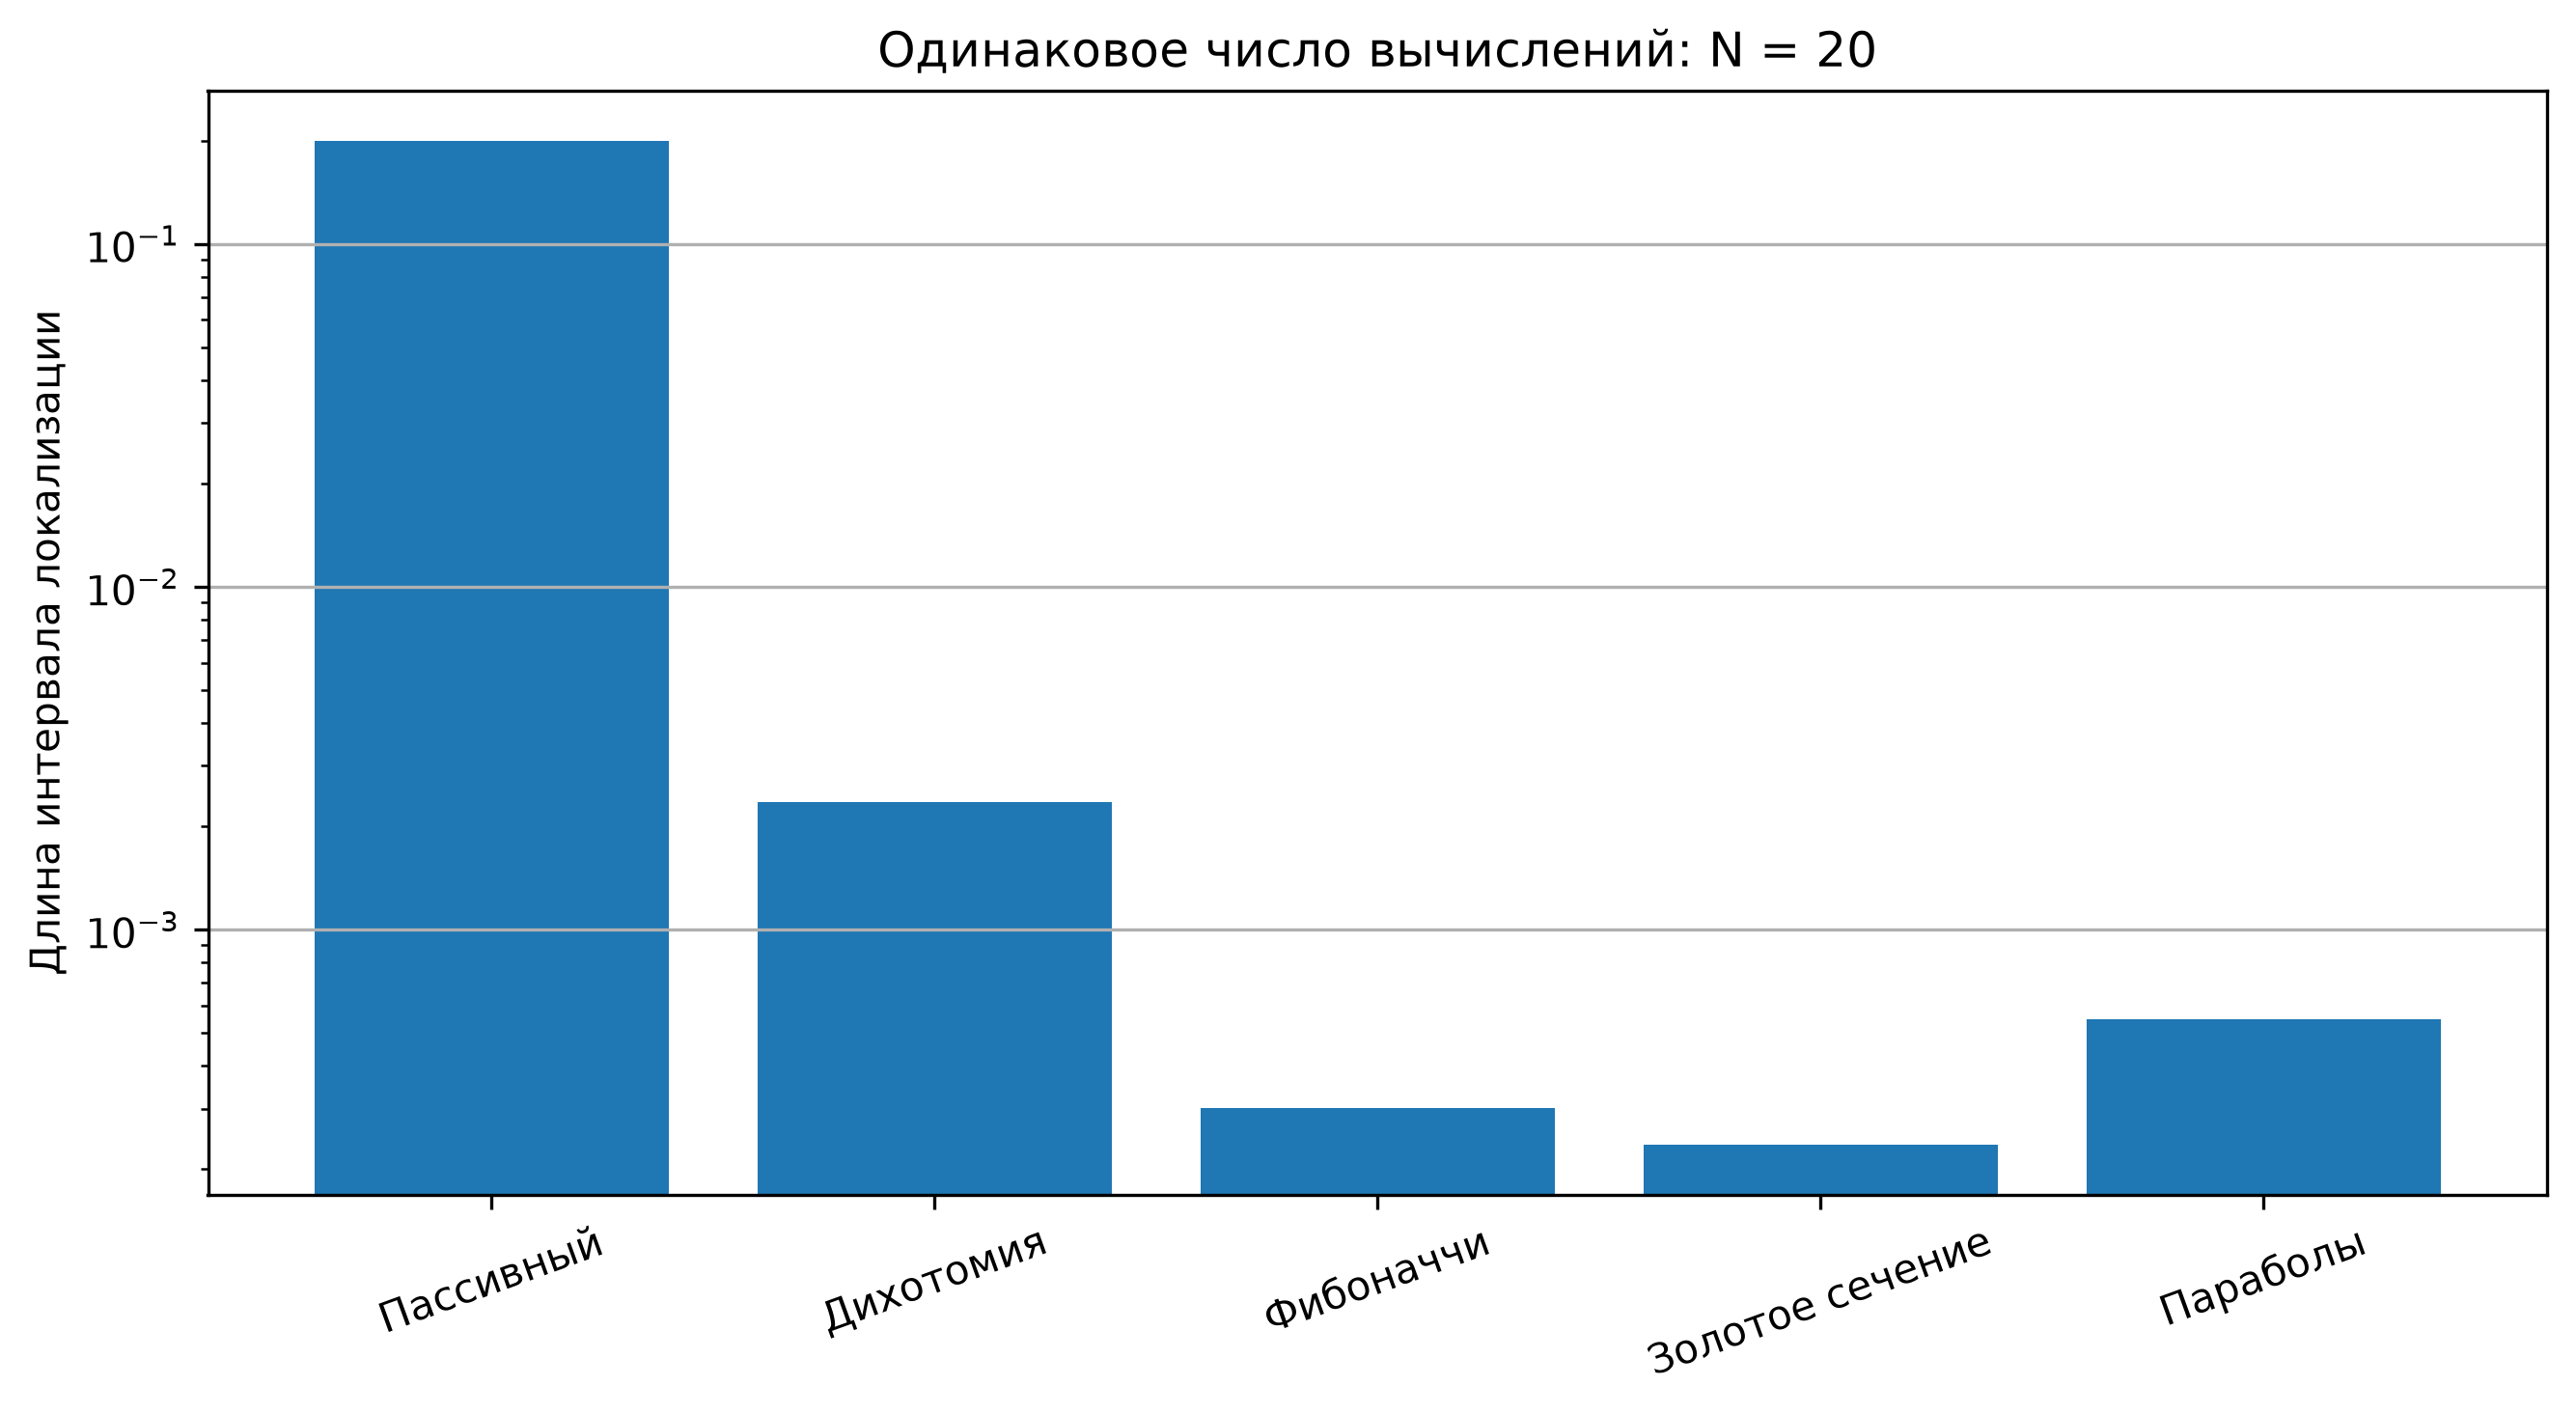
\includegraphics[width=0.88\textwidth]{results/comparison/local_f2.png}
	\caption{Сравнение длины итогового интервала при одинаковом числе вычислений для $f_2$.}
	\label{fig:local-comparison-f2}
\end{figure}

\newpage
